\documentclass[flegn]{beamer}
\usepackage{epsfig,dsfont,natbib}
\usepackage{xcolor}
\usepackage{graphicx,pgf}
\mode<presentation>

\usepackage{fancyhdr,lastpage,setspace}
\pagestyle{fancy} \fancyhf{} 
\rfoot{\vspace{-0.5cm}
\scriptsize{\thepage}}


\renewcommand\headrulewidth{0pt}
\newcommand{\dbl}{\setstretch{1.25}}
\newcommand{\hlf}{\setstretch{1}}


\newcommand{\bl}{\color{blue}}
\newcommand{\rd}{\color{red}}
\newcommand{\bk}{\color{black}}
\newcommand{\gr}{\color{green}}

\newcommand{\bs}[1]{\boldsymbol{#1}}
\newcommand{\mc}[1]{\mathcal{#1}}
\newcommand{\mr}[1]{\mathrm{#1}}
\newcommand{\bm}[1]{\mathbf{#1}}
\newcommand{\ds}[1]{\mathds{#1}}

\newcommand{\bi}{\begin{itemize}}
\newcommand{\ib}{\end{itemize}}
\newcommand{\p}{\item}
\newcommand{\sk}{\vspace{.5cm}}
\newcommand{\be}{\begin{enumerate}[(i)]}
\newcommand{\eb}{\end{enumerate}}


\newcommand{\sko}{\vspace{.1in}}
\newcommand{\skoo}{\vspace{.2in}}
\newcommand{\skooo}{\vspace{.3in}}
\newcommand{\hko}{\hspace{.1in}}
\newcommand{\hkoo}{\hspace{.2in}}
\newcommand{\hkooo}{\hspace{.3in}}

\newcommand{\gvn}{\; | \;}

\newcommand{\E}{\ds{E}}
\newcommand{\var}{\mr{var}}


%\usepackage{textpos}
%\addtobeamertemplate{frametitle}{}{%
%\begin{textblock*}{100mm}(.83\textwidth,-0.8cm)
%\includegraphics[width=2.8cm]{CLEE}
%\end{textblock*}}
\begin{document}

\title{ 
\includegraphics[width=3in]{LogoMSBA.png} \\ \vskip .5cm {\bf Introduction to Predictive Models} \\ Book Chapters 1, 2 and 5.}

\author{ \small
	  {\bf Carlos M.  Carvalho} \\ The University of Texas McCombs School of Business\\}
%  \vskip .2cm \texttt{mccombs.utexas.edu/faculty/carlos.carvalho/teaching} \\  \vspace{0.5cm}  \includegraphics[width=1.8in]{CLEE.png}}


\date{}
\maketitle

\dbl


%Table of Contents
\setcounter{page}{0}
\thispagestyle{empty}
\begin{minipage}{5.in}
\vspace{1.0in}
\tableofcontents
\end{minipage}
\newpage

\section{\arabic{section}. Introduction}
%%%%%%%%%%%%%%%%%%%%%%%%%%%%%%%
\begin{frame}
\frametitle{\arabic{section}. Introduction to Predictive Models}

Simply put, the goal is to predict a \\ {\color{red}target variable $Y$} with {\color{blue}input variables $X$}! 

\skoo

In Data Mining terminology this is know as {\bf supervised learning} (also called {\it Predictive Analytics}).

\skoo
In general, a useful way to think about it is  that $Y$ and $X$ are related in the following way:
$$
Y_i =f(X_i) + \epsilon_i
$$

\skoo
{\color{blue}The main purpose of this part of the course is to {\it learn or estimate} $f(\cdot)$ from data }

\end{frame}



%%%%%%%%%%%%%%%%%%%%%%%%%%%%%%%
\begin{frame}
\frametitle{Example: Boston Housing}
We might be interested in predicting the median house value as a function of some measure of social economic level... here's some data:
\vspace{-0.9cm}
\begin{center}
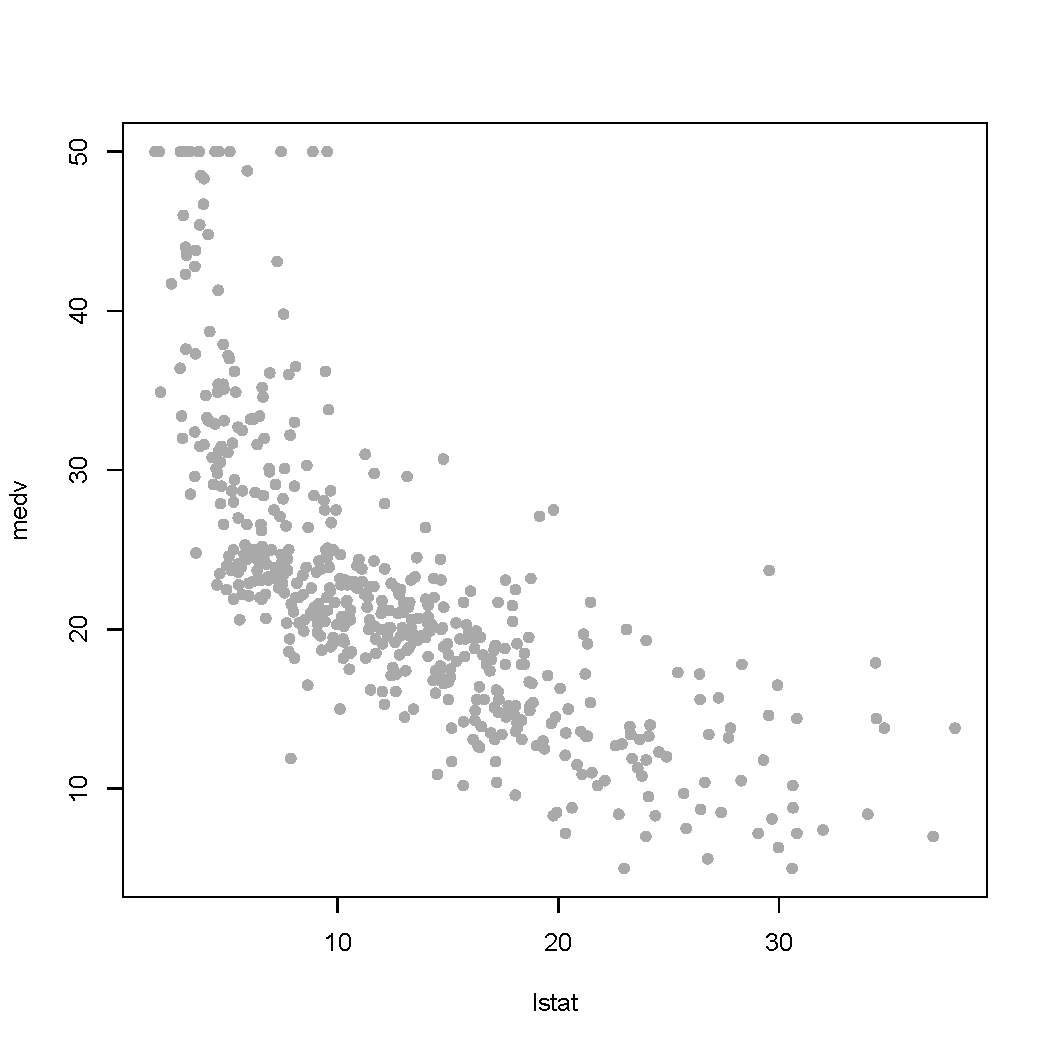
\includegraphics[width=3in]{Boston1}
\end{center}
\vspace{-1cm}
{\color{red}What should $f(\cdot)$ be?}
\end{frame}



%%%%%%%%%%%%%%%%%%%%%%%%%%%%%%%
\begin{frame}
\frametitle{Example: Boston Housing}
How about this...
\vspace{-0.8cm}
\begin{center}
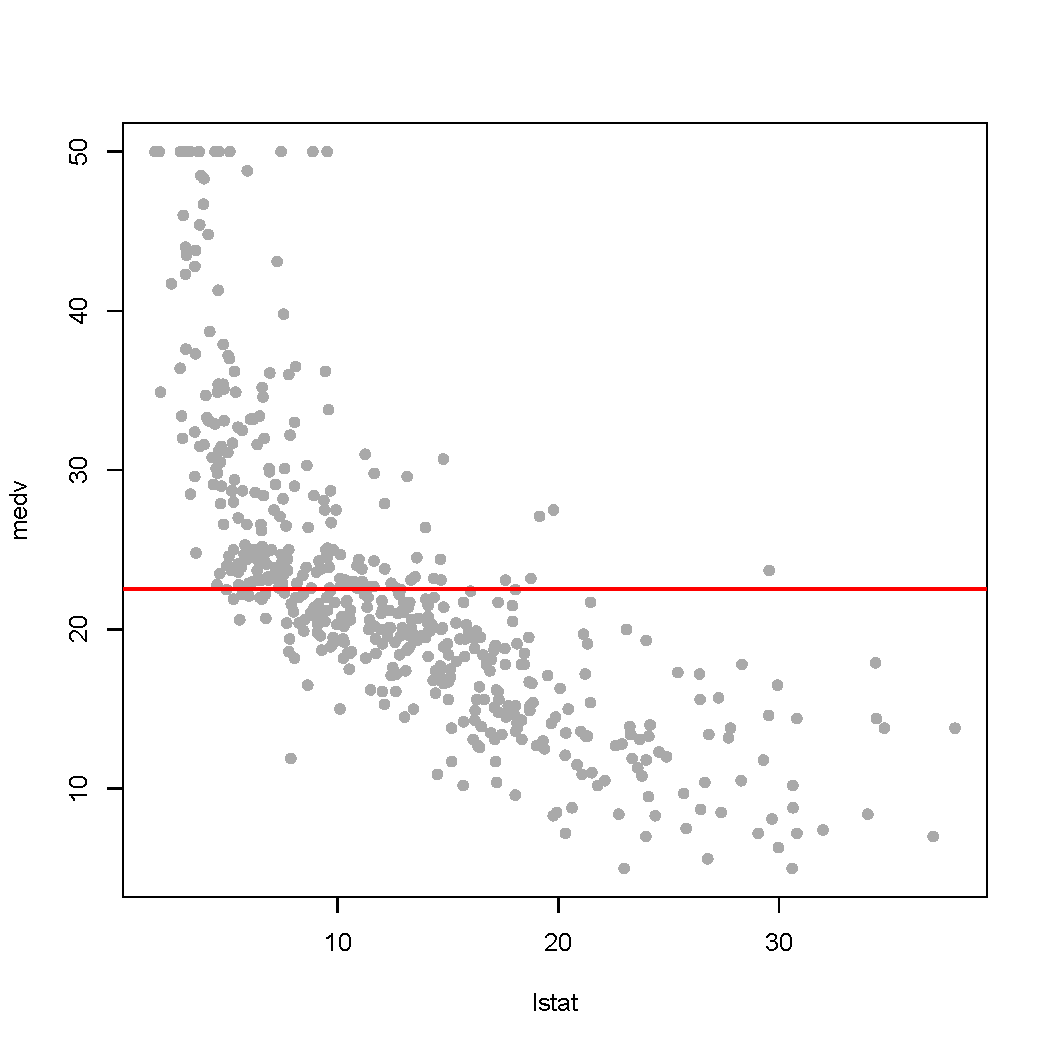
\includegraphics[width=3in]{Boston2}
\end{center}

\vspace{-0.5cm}
{\color{red}If $lstat=30$ what is the prediction for $medv$?}
\end{frame}


%%%%%%%%%%%%%%%%%%%%%%%%%%%%%%%
\begin{frame}
\frametitle{Example: Boston Housing}
or this...
\vspace{-0.8cm}
\begin{center}
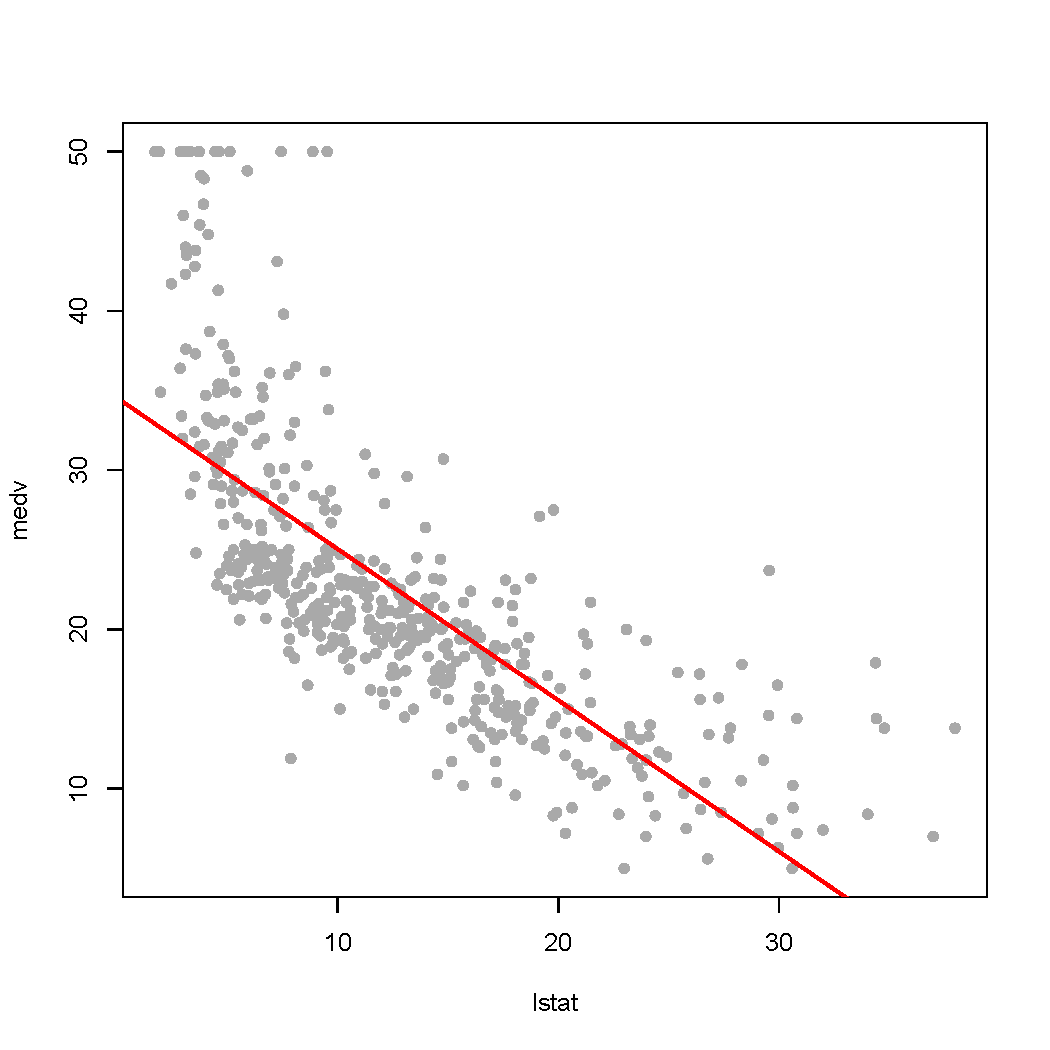
\includegraphics[width=3in]{Boston3}
\end{center}

\vspace{-0.5cm}
{\color{red}If $lstat=30$ what is the prediction for $medv$?}
\end{frame}


%%%%%%%%%%%%%%%%%%%%%%%%%%%%%%%
\begin{frame}
\frametitle{Example: Boston Housing}
or even this?
\vspace{-0.8cm}
\begin{center}
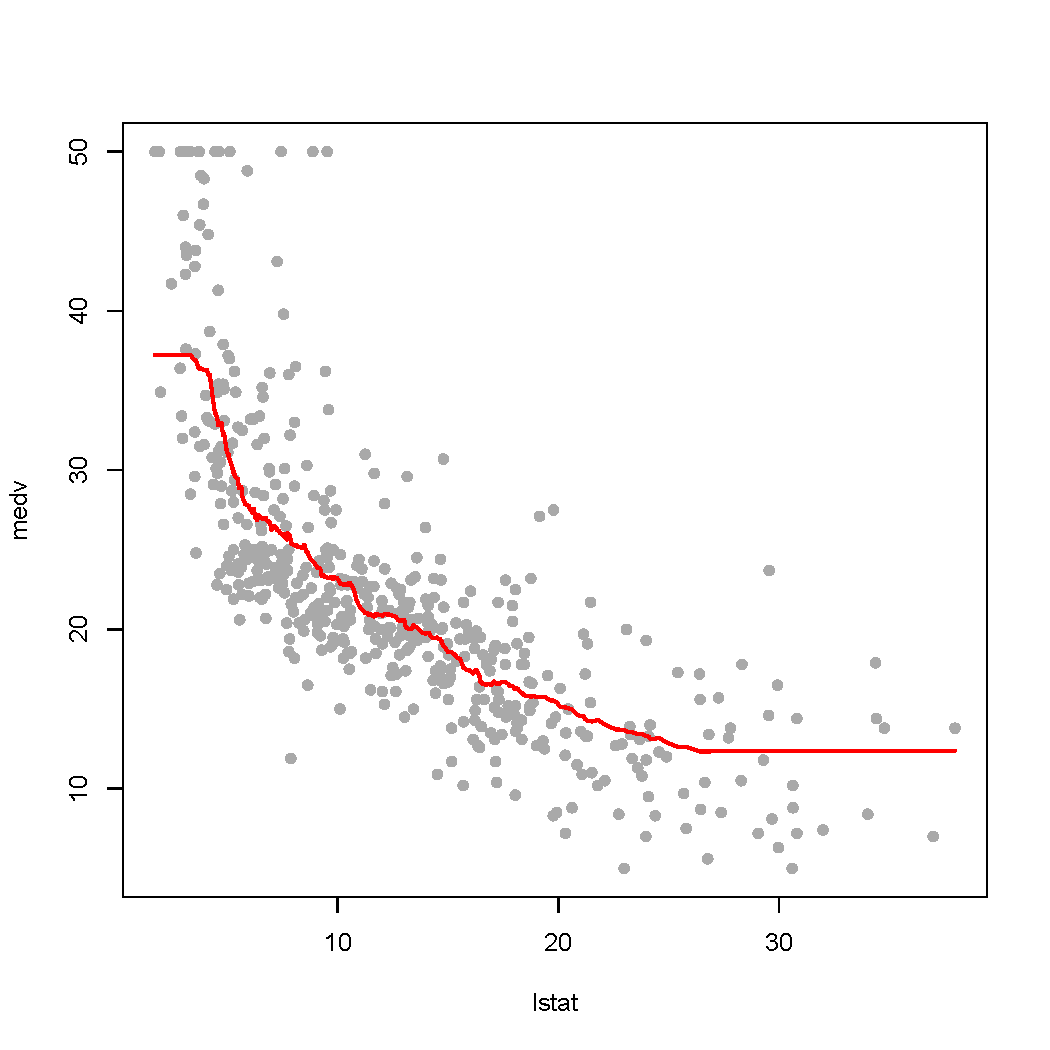
\includegraphics[width=3in]{Boston4}
\end{center}

\vspace{-0.5cm}
{\color{red}If $lstat=30$ what is the prediction for $medv$?}
\end{frame}

%%%%%%%%%%%%%%%%%%%%%%%%%%%%%%%
\begin{frame}
\frametitle{How do we estimate $f(\cdot)$?}
\begin{itemize}
\item Using {\color{red}{\it training data}}:
$$
\left\{ (X_1, Y_1), (X_2,Y_2), \dots, (X_n,Y_n) \right\}
$$
\item We use a statistical method to {\color{red}{\it estimate}} the function $f(\cdot)$
\item Two general methodological strategies:
\begin{enumerate}
\item parametric models (restricted assumptions about $f(\cdot)$)
\item non-parametric models (flexibility in defining $f(\cdot)$)
\end{enumerate}
\end{itemize}
\begin{tabular}{lr}
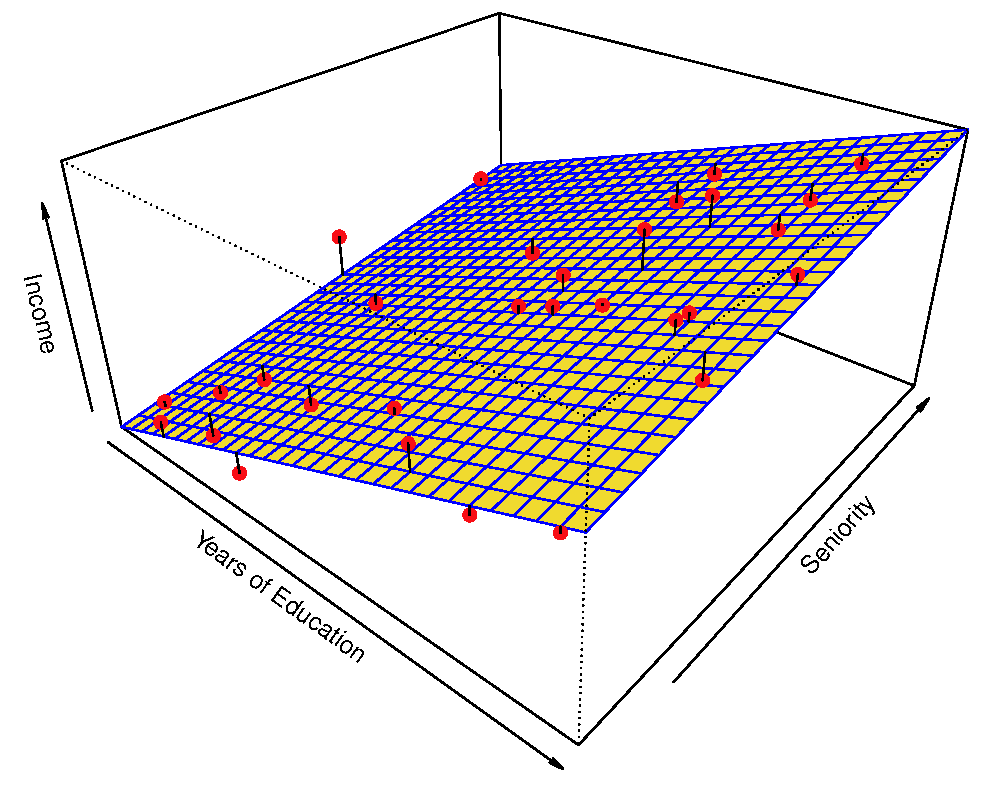
\includegraphics[width=1.8in]{Gareth2-4.pdf}&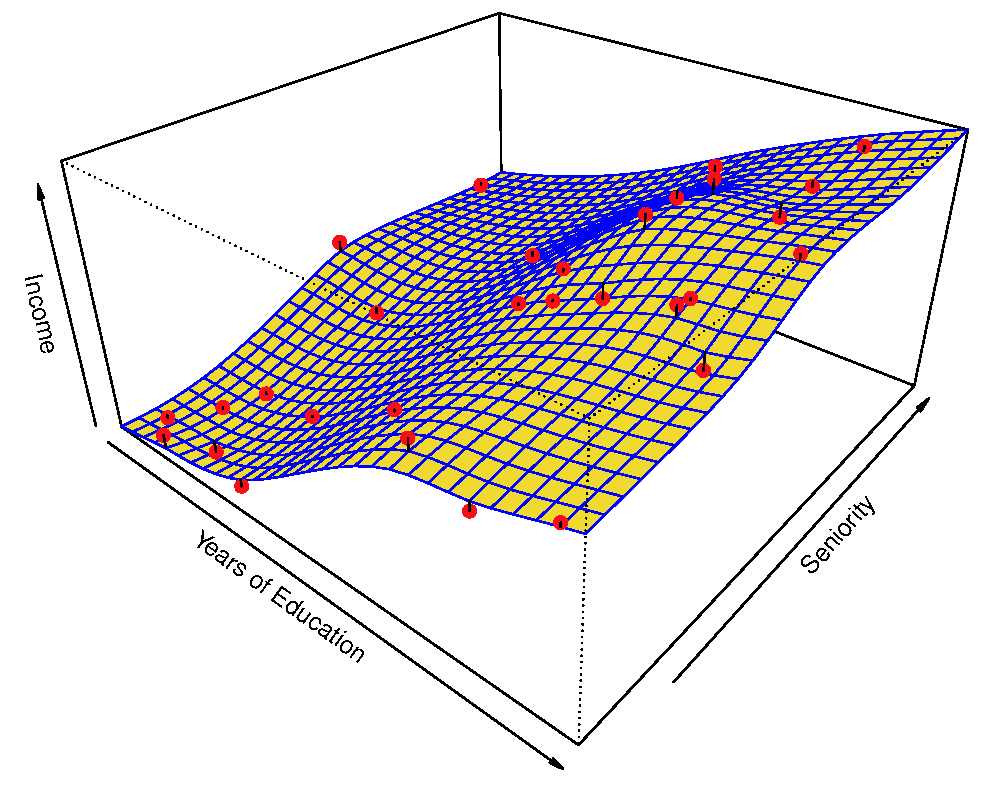
\includegraphics[width=1.8in]{Gareth2-5.pdf}
\end{tabular}
\end{frame}



%%%%%%%%%%%%%%%%%%%%%%%%%%%%%%%
\begin{frame}
\frametitle{Back to Boston Housing}
\begin{tabular}{ll}
Parametric Model  & Non-Parametric Model   \\
 ($Y=\mu+\epsilon$)&(k-nearest neighbors)\\
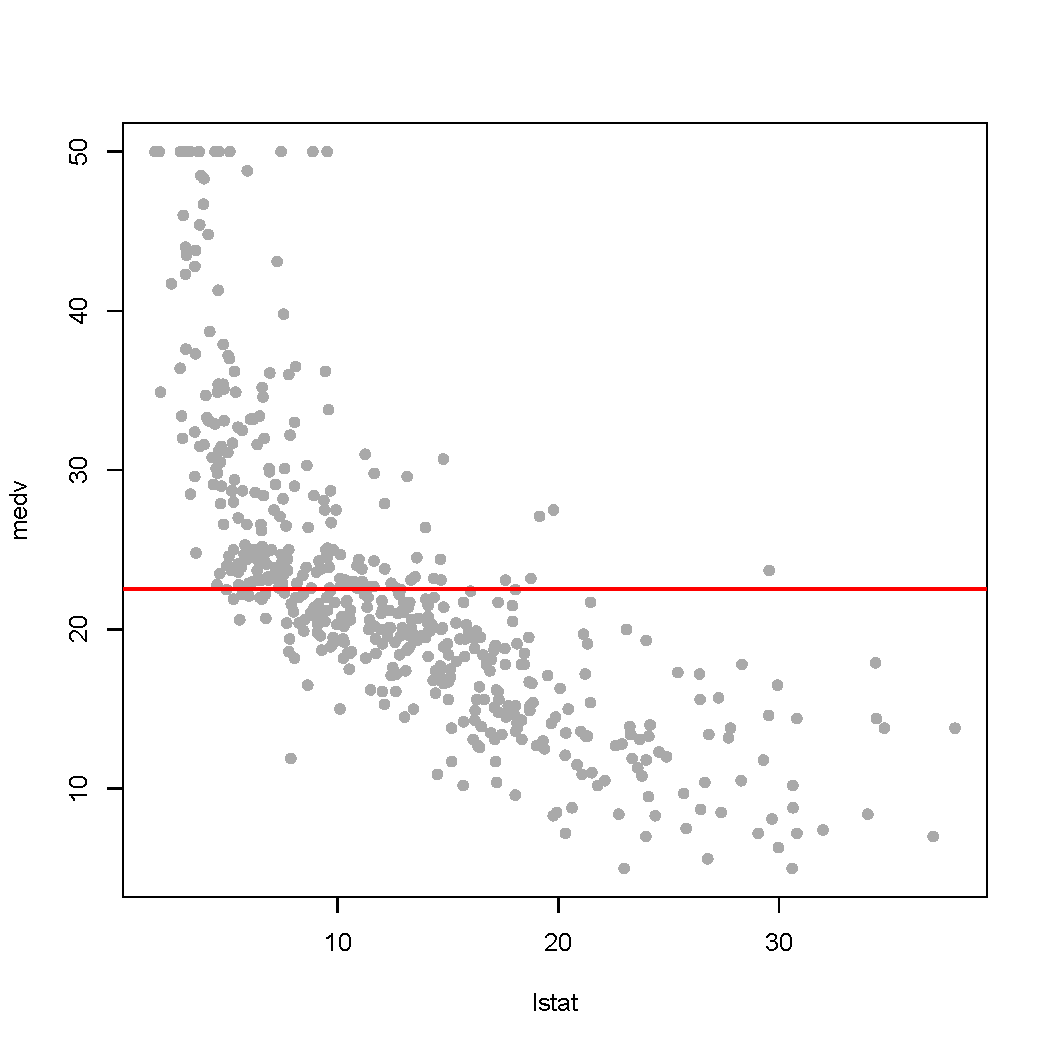
\includegraphics[width=2.1in]{Boston2}&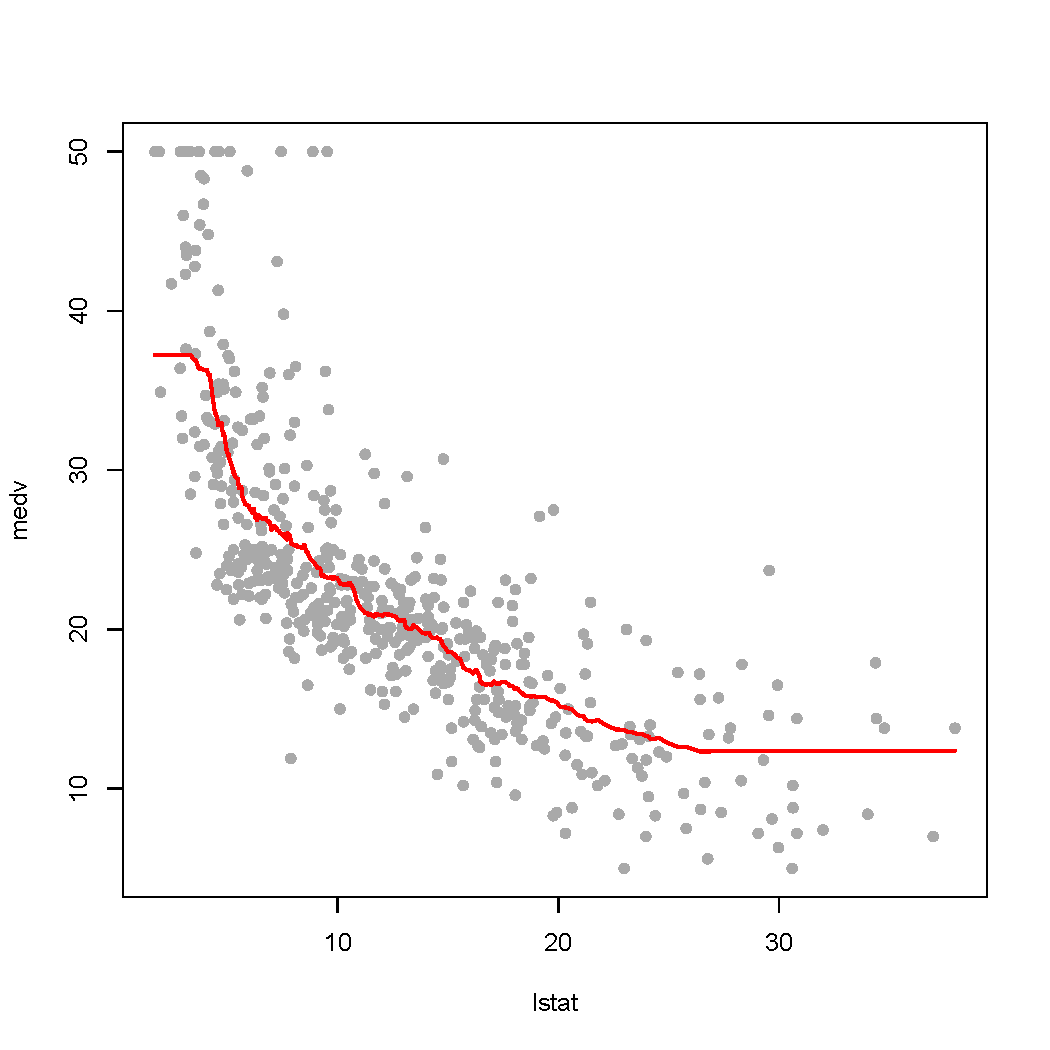
\includegraphics[width=2.1in]{Boston4}
\end{tabular}
\end{frame}

%%%%%%%%%%%%%%%%%%%%%%%%%%%%%%%
\begin{frame}
\frametitle{Back to Boston Housing}
Simplest parametric model:
$$
Y_i  = \mu + \epsilon_i
$$

\sko

\begin{minipage}{2.3in}
Using the training data, we estimate $f(\cdot)$ as
$$
\widehat{f(\cdot)} = \hat{\mu} = \bar{Y} = \frac{1}{n}\sum_{i=1}^n Y_i
$$
\end{minipage}
\begin{minipage}{1.65in}
\begin{center}
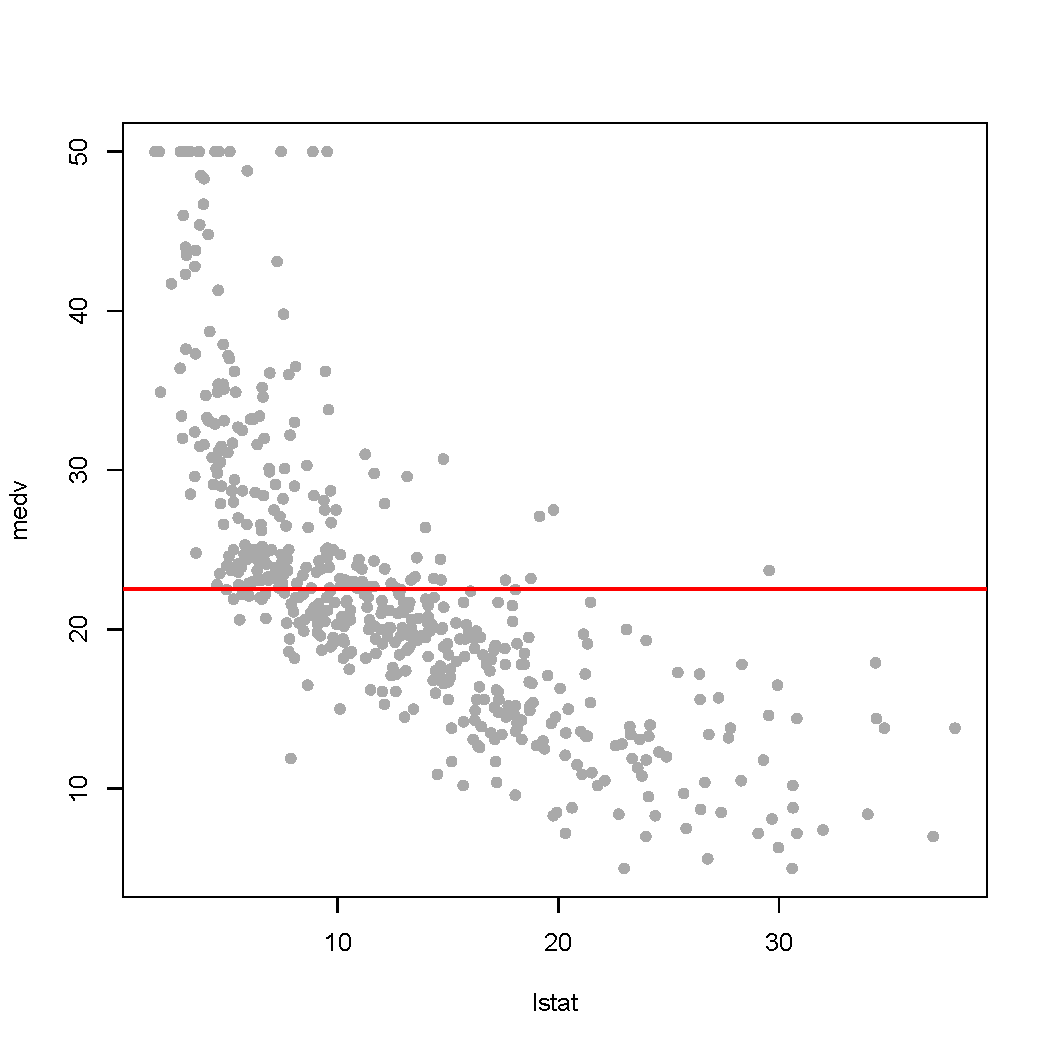
\includegraphics[width=2.1in]{Boston2}
\end{center}
\end{minipage}
\end{frame}

%%%%%%%%%%%%%%%%%%%%%%%%%%%%%%%
\begin{frame}
\frametitle{Back to Boston Housing}
The above strategy averages all points in the training set... maybe points that are {\color{blue}``closer''} to the place I am trying to predict should be more relevant... 

\sko

How about averaging the closest 20 neighbors?  \\ {\color{red}What do I mean by closest?} We will choose the 20 points that are closest to the $X$ value we are trying to predict.

\sko

This is what is called the {\color{blue}$k$-nearest neighbors} algorithm

\end{frame}


%%%%%%%%%%%%%%%%%%%%%%%%%%%%%%%
\begin{frame}
\frametitle{Back to Boston Housing}

\vspace{-0.7cm}
\begin{center}
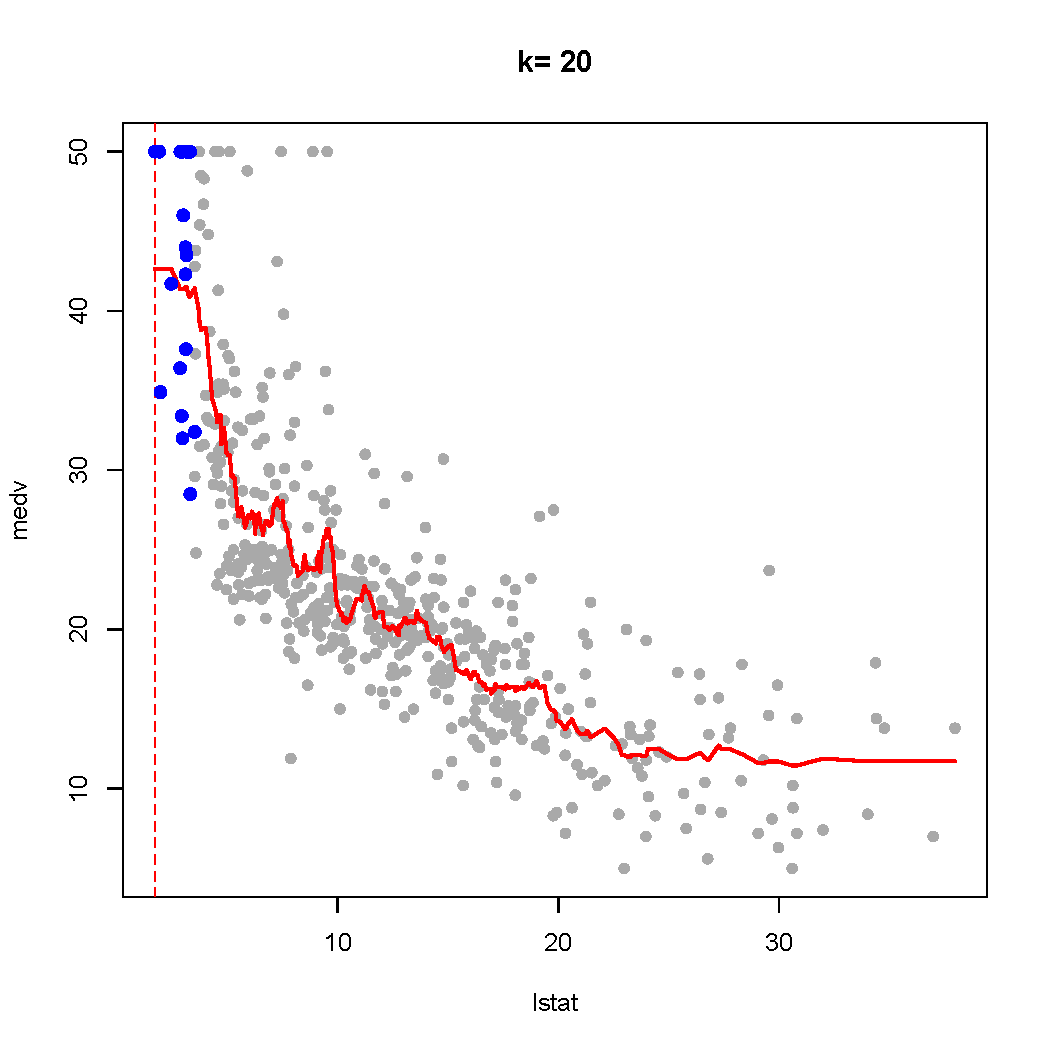
\includegraphics[width=3in]{k20-1}
\end{center}
\end{frame}

%%%%%%%%%%%%%%%%%%%%%%%%%%%%%%%
\begin{frame}
\frametitle{Back to Boston Housing}

\vspace{-0.7cm}
\begin{center}
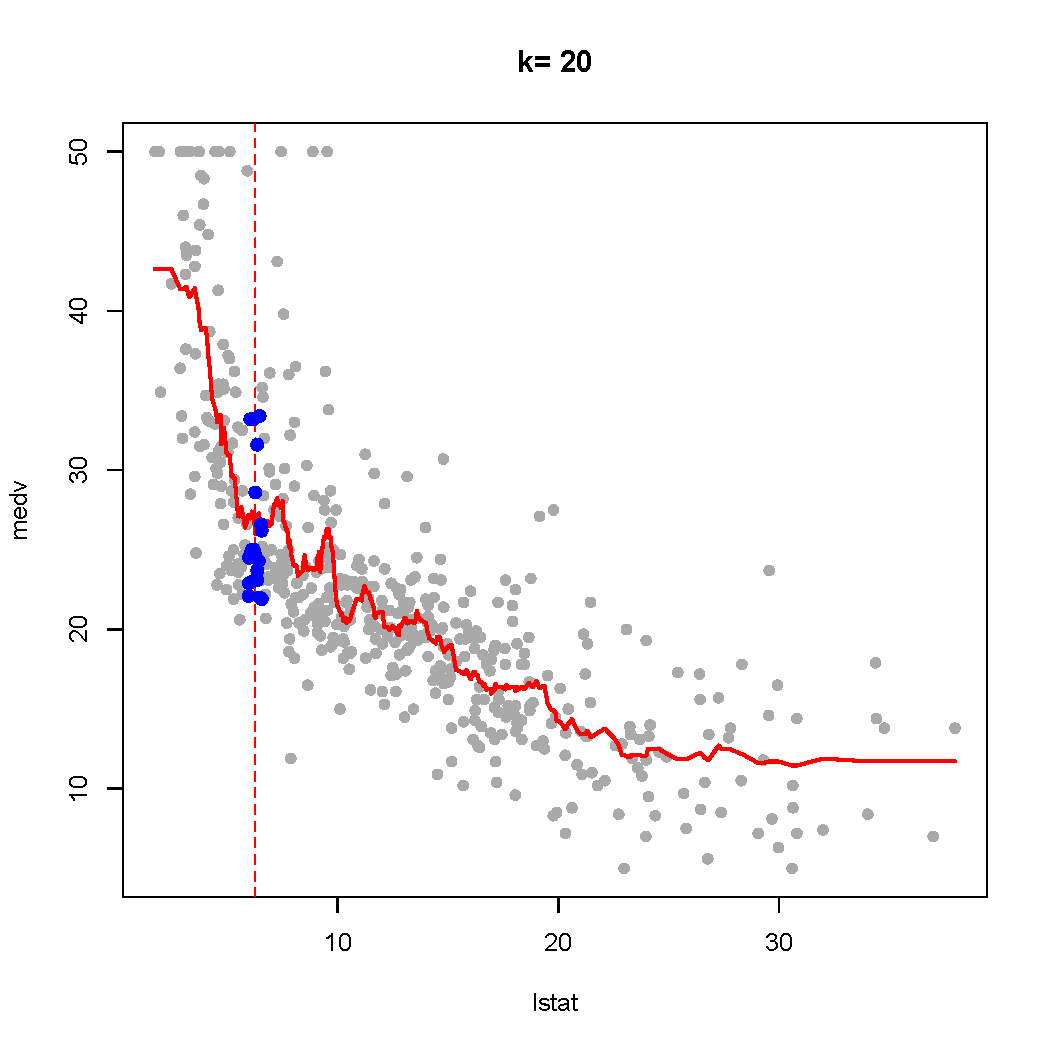
\includegraphics[width=3in]{k20-2}
\end{center}
\end{frame}
%%%%%%%%%%%%%%%%%%%%%%%%%%%%%%%
\begin{frame}
\frametitle{Back to Boston Housing}

\vspace{-0.7cm}
\begin{center}
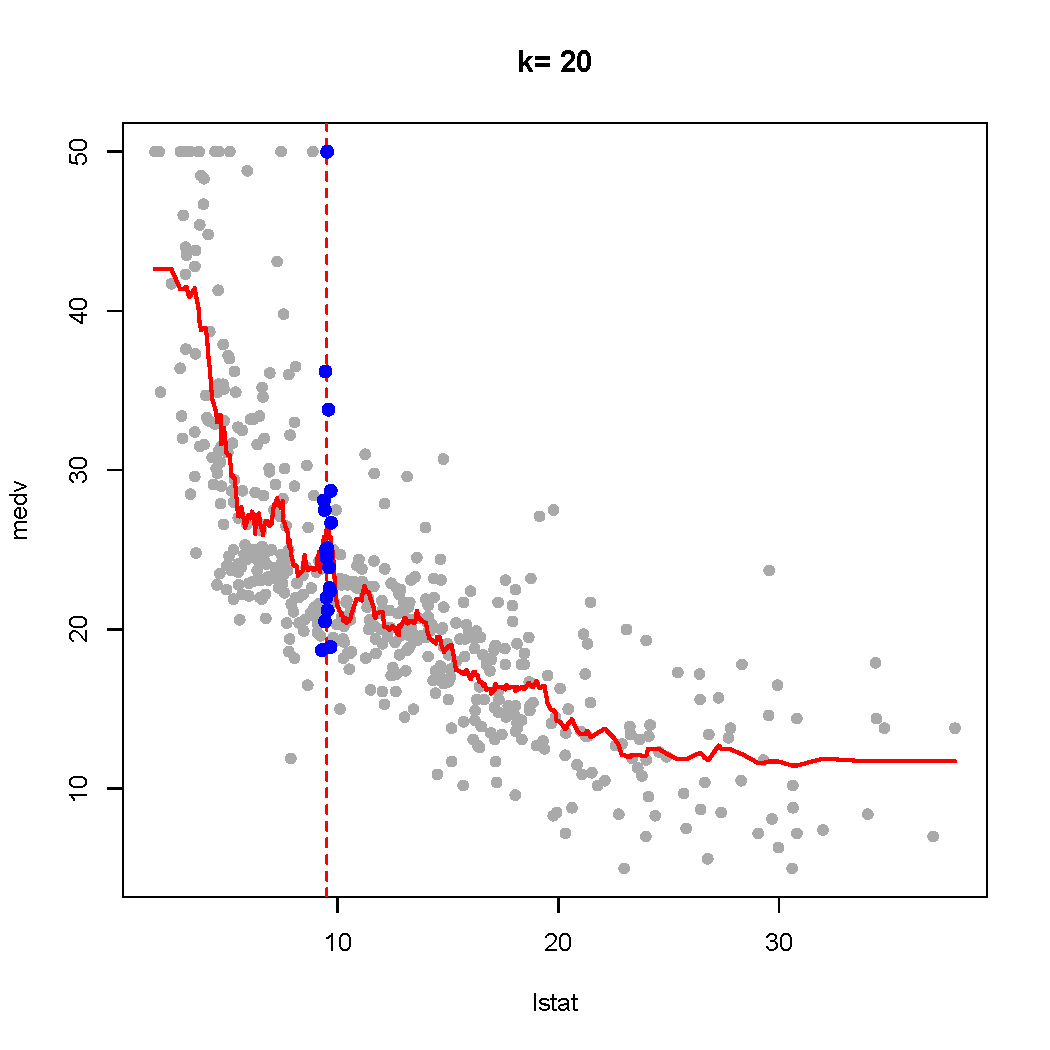
\includegraphics[width=3in]{k20-3}
\end{center}
\end{frame}
%%%%%%%%%%%%%%%%%%%%%%%%%%%%%%%
\begin{frame}
\frametitle{Back to Boston Housing}
\vspace{-0.7cm}
\begin{center}
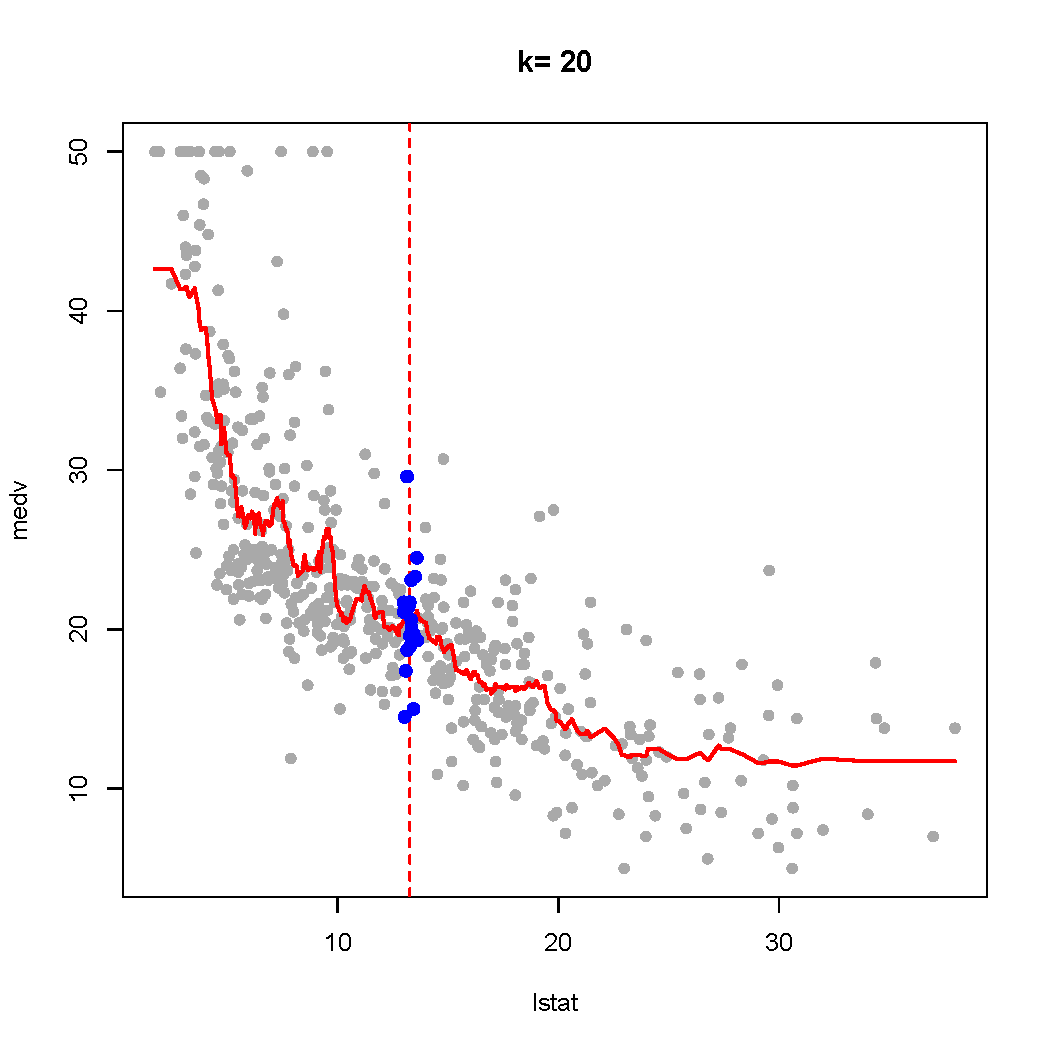
\includegraphics[width=3in]{k20-4}
\end{center}
\end{frame}
%%%%%%%%%%%%%%%%%%%%%%%%%%%%%%%
\begin{frame}
\frametitle{Back to Boston Housing}

\vspace{-0.7cm}
\begin{center}
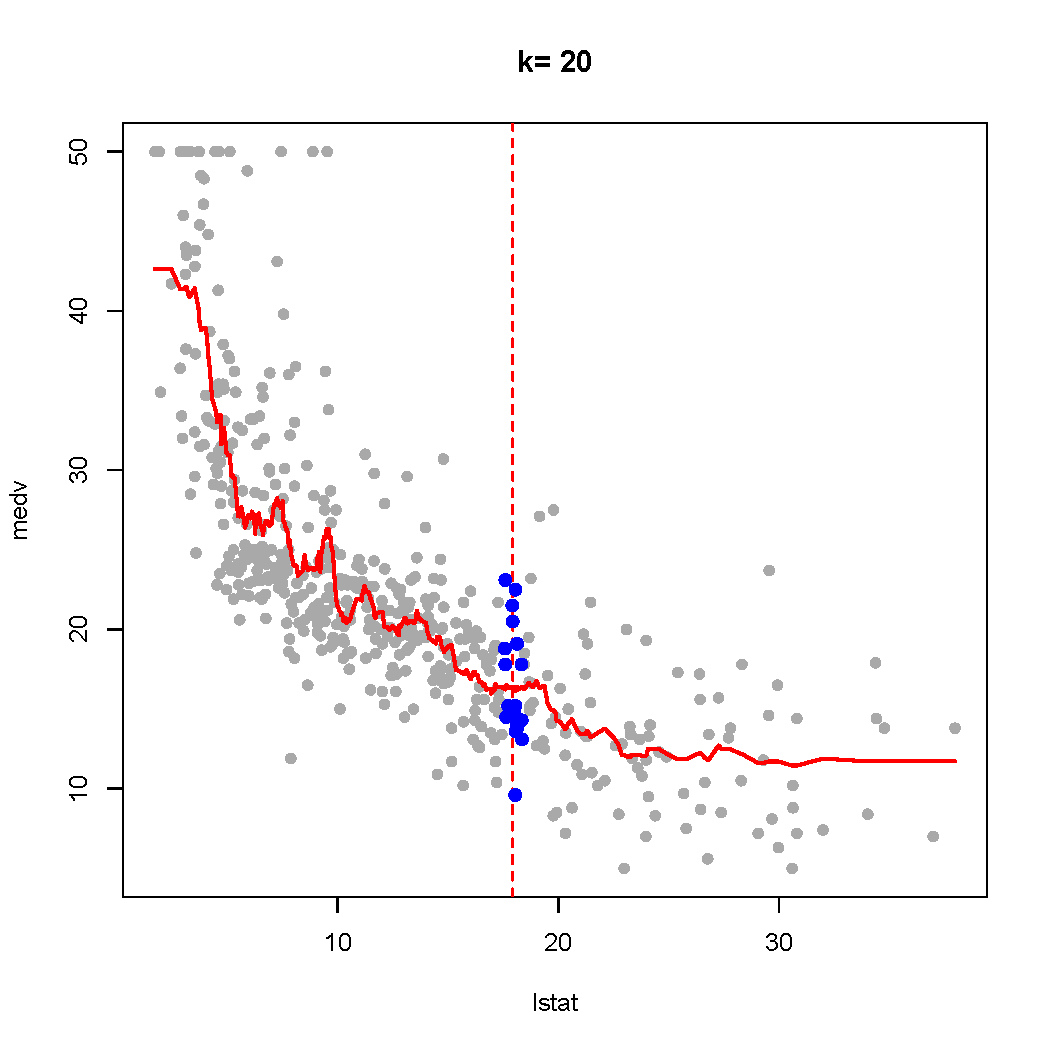
\includegraphics[width=3in]{k20-5}
\end{center}
\end{frame}
%%%%%%%%%%%%%%%%%%%%%%%%%%%%%%%
\begin{frame}
\frametitle{Back to Boston Housing}
\vspace{-0.7cm}
\begin{center}
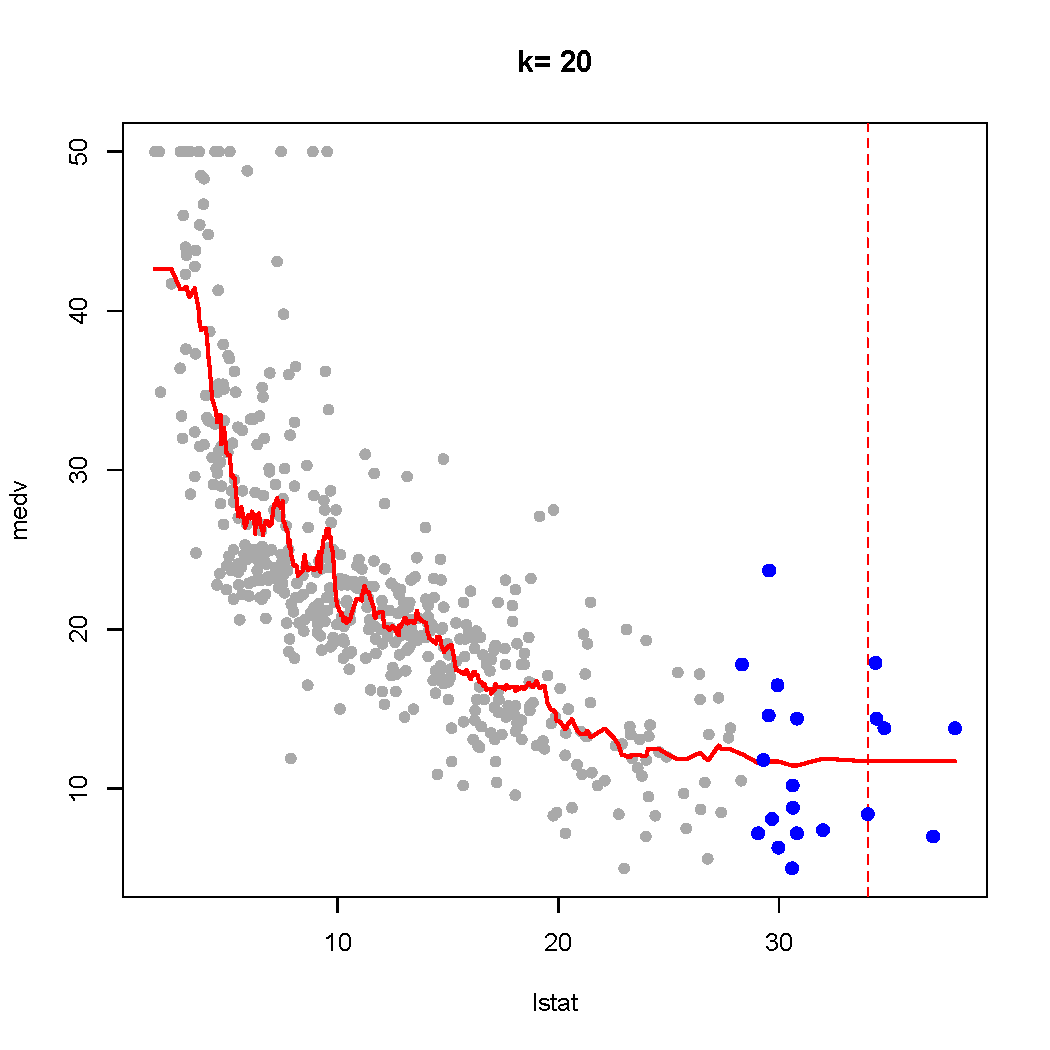
\includegraphics[width=3in]{k20-6}
\end{center}
\end{frame}



%%%%%%%%%%%%%%%%%%%%%%%%%%%%%%%
\begin{frame}
\frametitle{Back to Boston Housing}
{\color{blue}Okay, that seems sensible but why not use 2 neighbors or 200 neighbors? }

\vspace{-0.5cm}
\begin{center}
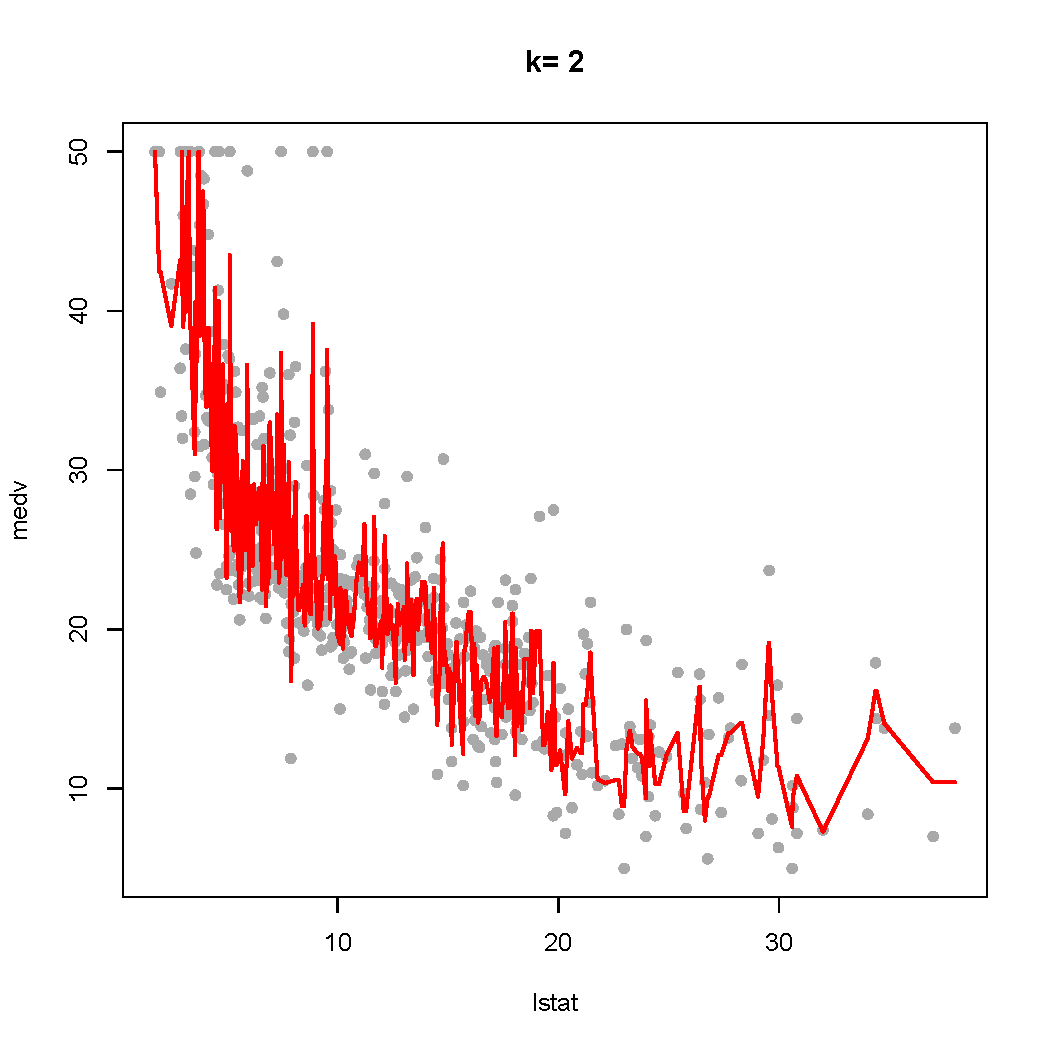
\includegraphics[width=3in]{k2}
\end{center}
\end{frame}


%%%%%%%%%%%%%%%%%%%%%%%%%%%%%%%
\begin{frame}
\frametitle{Back to Boston Housing}
{\color{blue}Okay, that seems sensible but why not use 5 neighbors or 200 neighbors? }

\vspace{-0.5cm}
\begin{center}
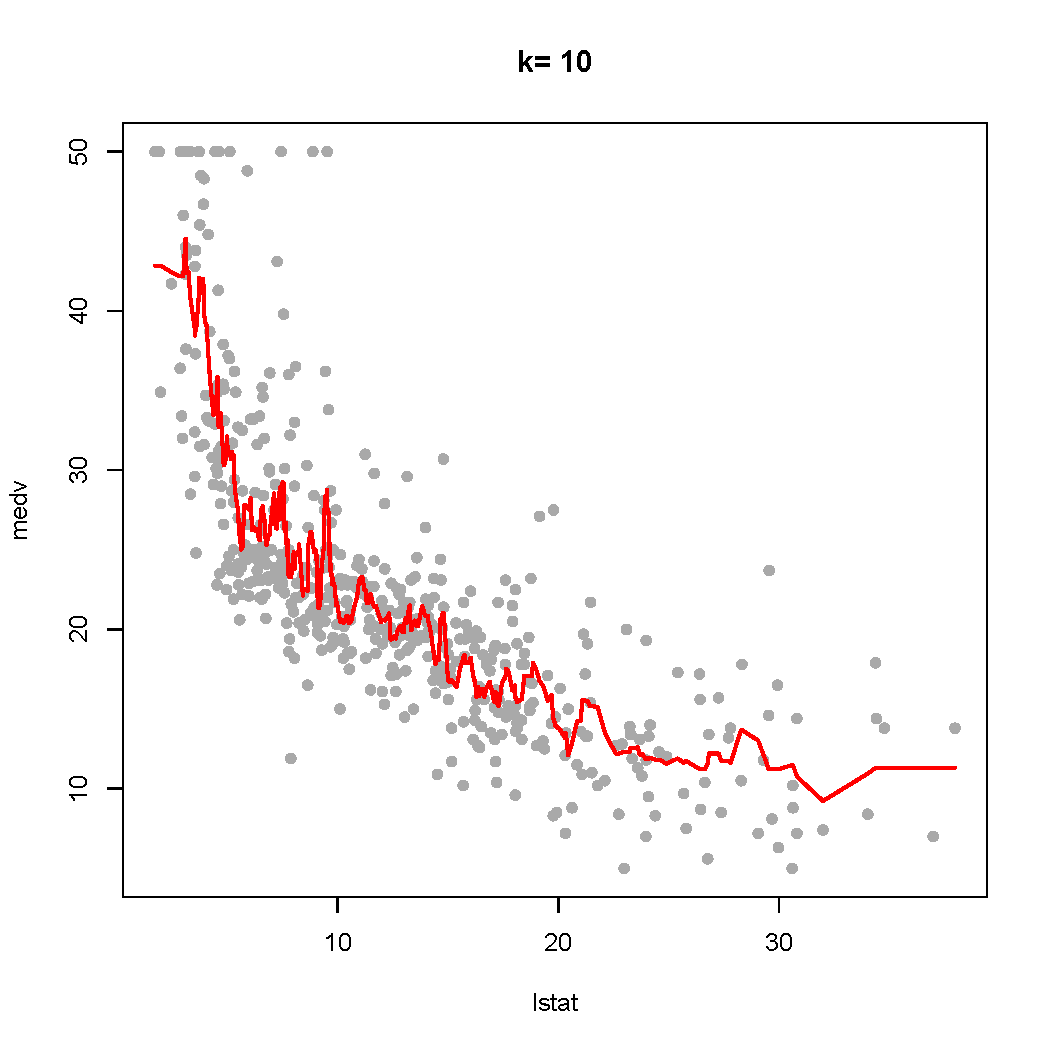
\includegraphics[width=3in]{k10}
\end{center}
\end{frame}


%%%%%%%%%%%%%%%%%%%%%%%%%%%%%%%
\begin{frame}
\frametitle{Back to Boston Housing}
{\color{blue}Okay, that seems sensible but why not use 5 neighbors or 200 neighbors? }

\vspace{-0.5cm}
\begin{center}
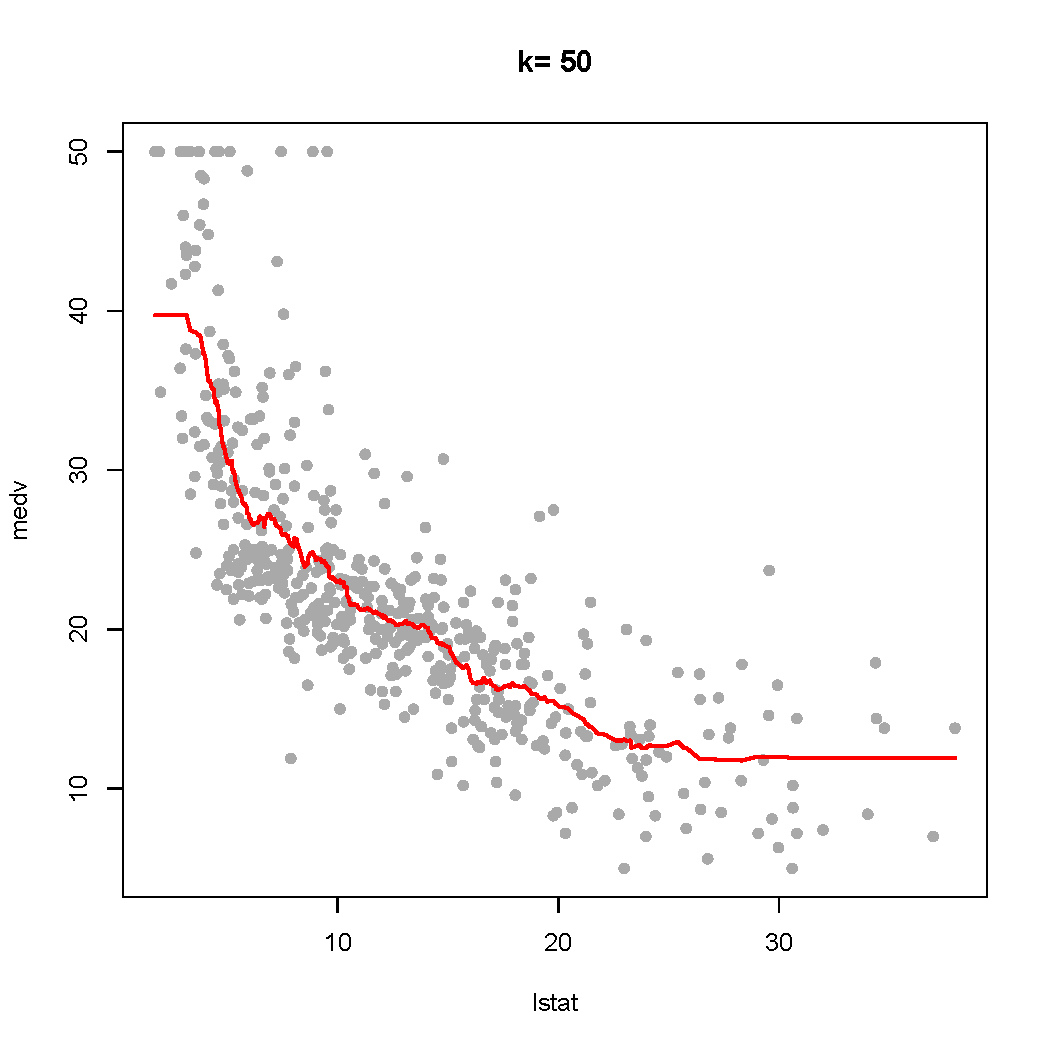
\includegraphics[width=3in]{k50}
\end{center}
\end{frame}

%%%%%%%%%%%%%%%%%%%%%%%%%%%%%%%
\begin{frame}
\frametitle{Back to Boston Housing}
{\color{blue}Okay, that seems sensible but why not use 5 neighbors or 200 neighbors? }

\vspace{-0.5cm}
\begin{center}
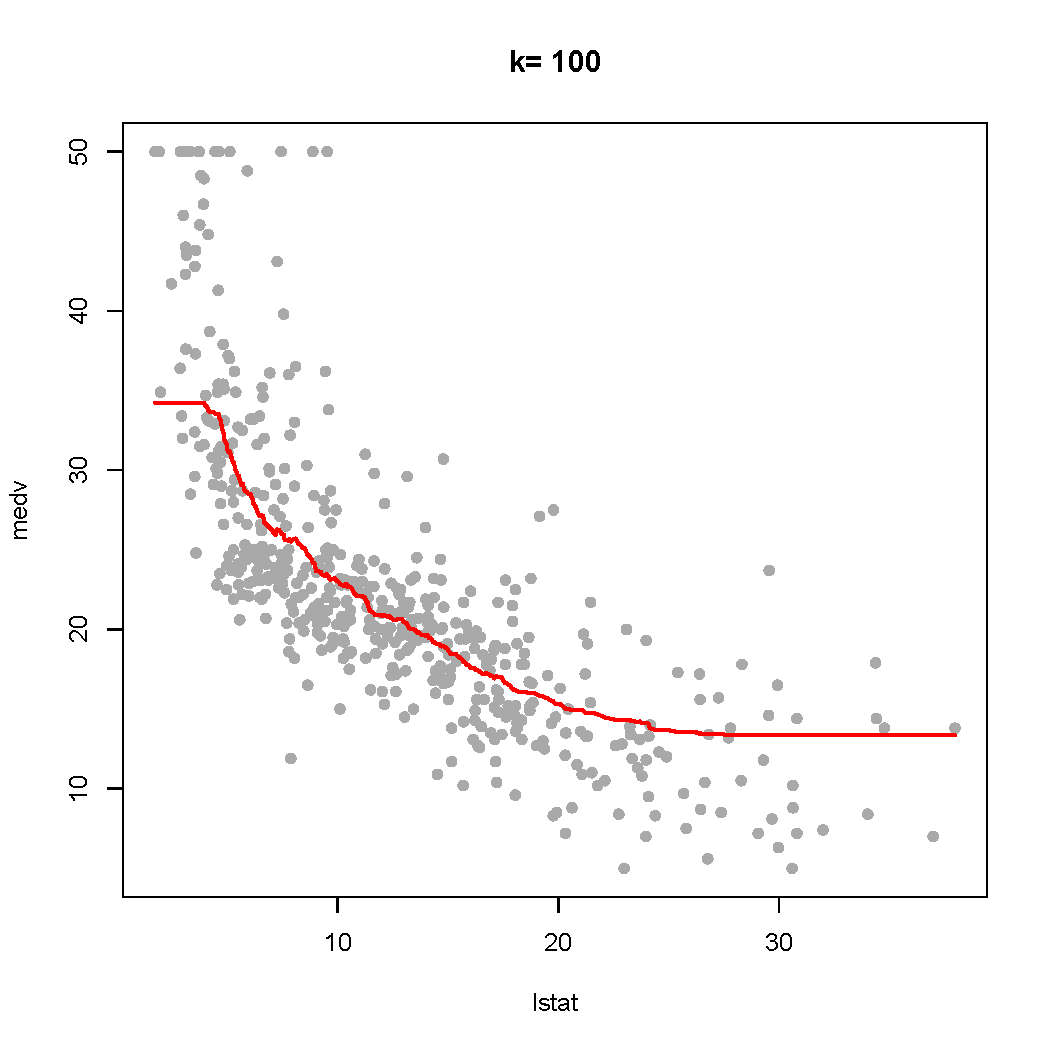
\includegraphics[width=3in]{k100}
\end{center}
\end{frame}

%%%%%%%%%%%%%%%%%%%%%%%%%%%%%%%
\begin{frame}
\frametitle{Back to Boston Housing}
{\color{blue}Okay, that seems sensible but why not use 5 neighbors or 200 neighbors? }

\vspace{-0.5cm}
\begin{center}
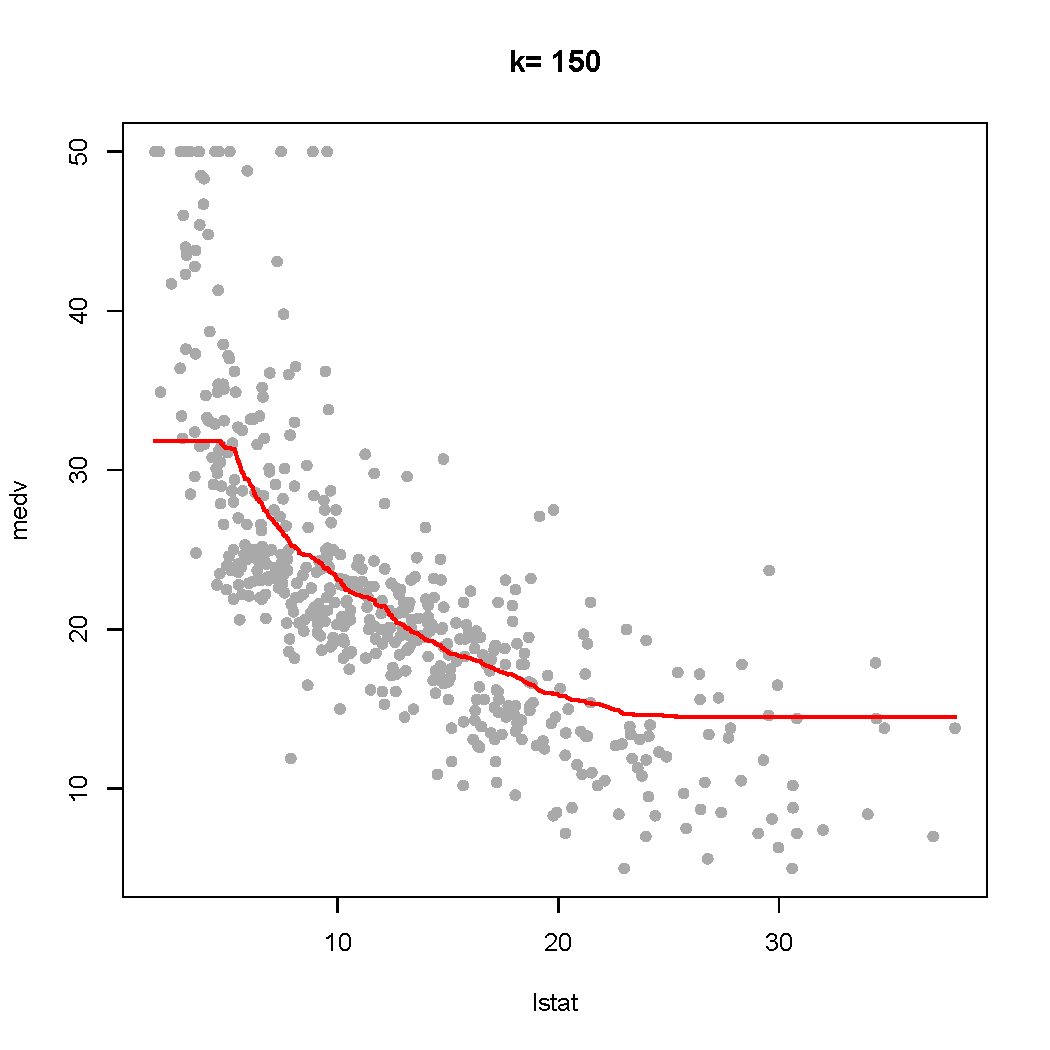
\includegraphics[width=3in]{k150}
\end{center}
\end{frame}

%%%%%%%%%%%%%%%%%%%%%%%%%%%%%%%
\begin{frame}
\frametitle{Back to Boston Housing}
{\color{blue}Okay, that seems sensible but why not use 5 neighbors or 200 neighbors? }

\vspace{-0.5cm}
\begin{center}
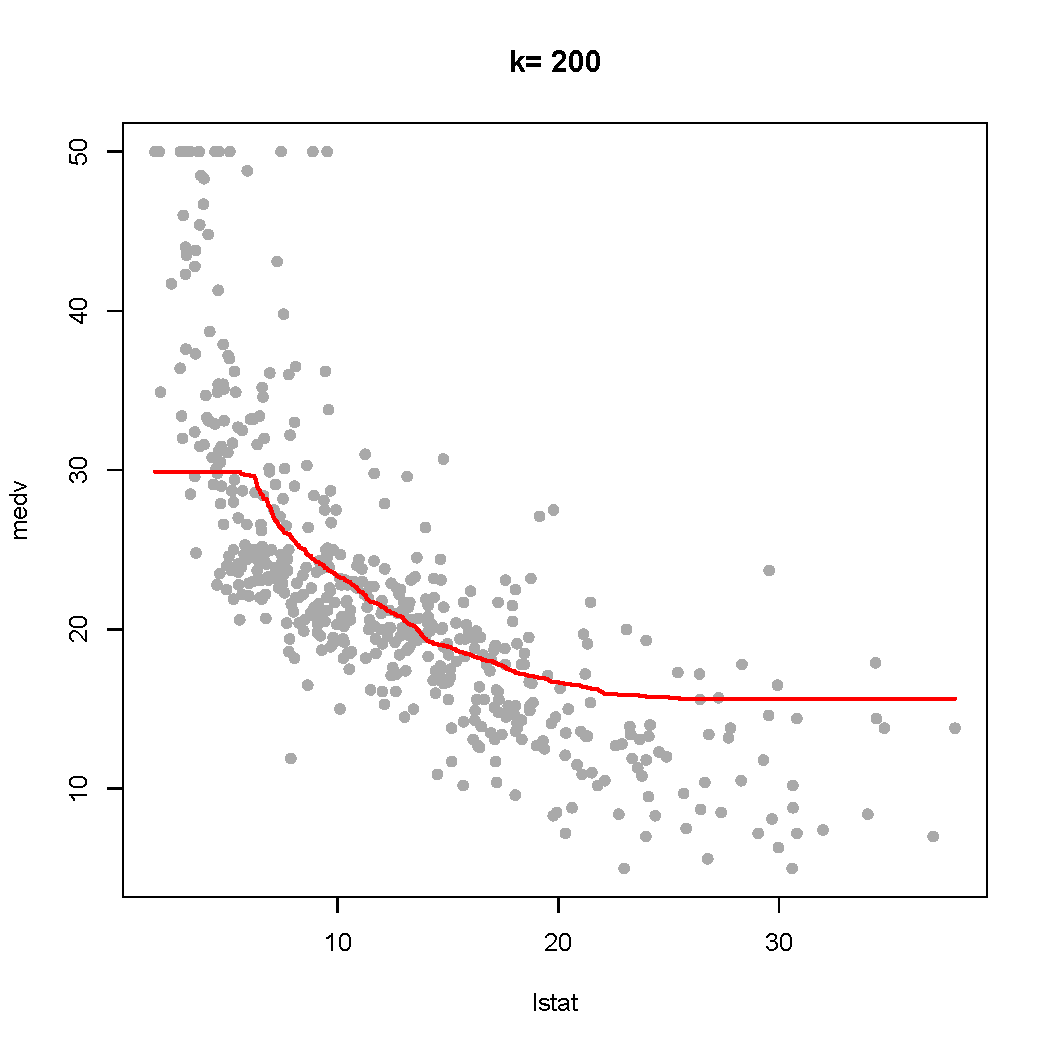
\includegraphics[width=3in]{k200}
\end{center}
\end{frame}

%%%%%%%%%%%%%%%%%%%%%%%%%%%%%%%
\begin{frame}
\frametitle{Back to Boston Housing}
{\color{blue}Okay, that seems sensible but why not use 5 neighbors or 200 neighbors? }

\vspace{-0.5cm}
\begin{center}
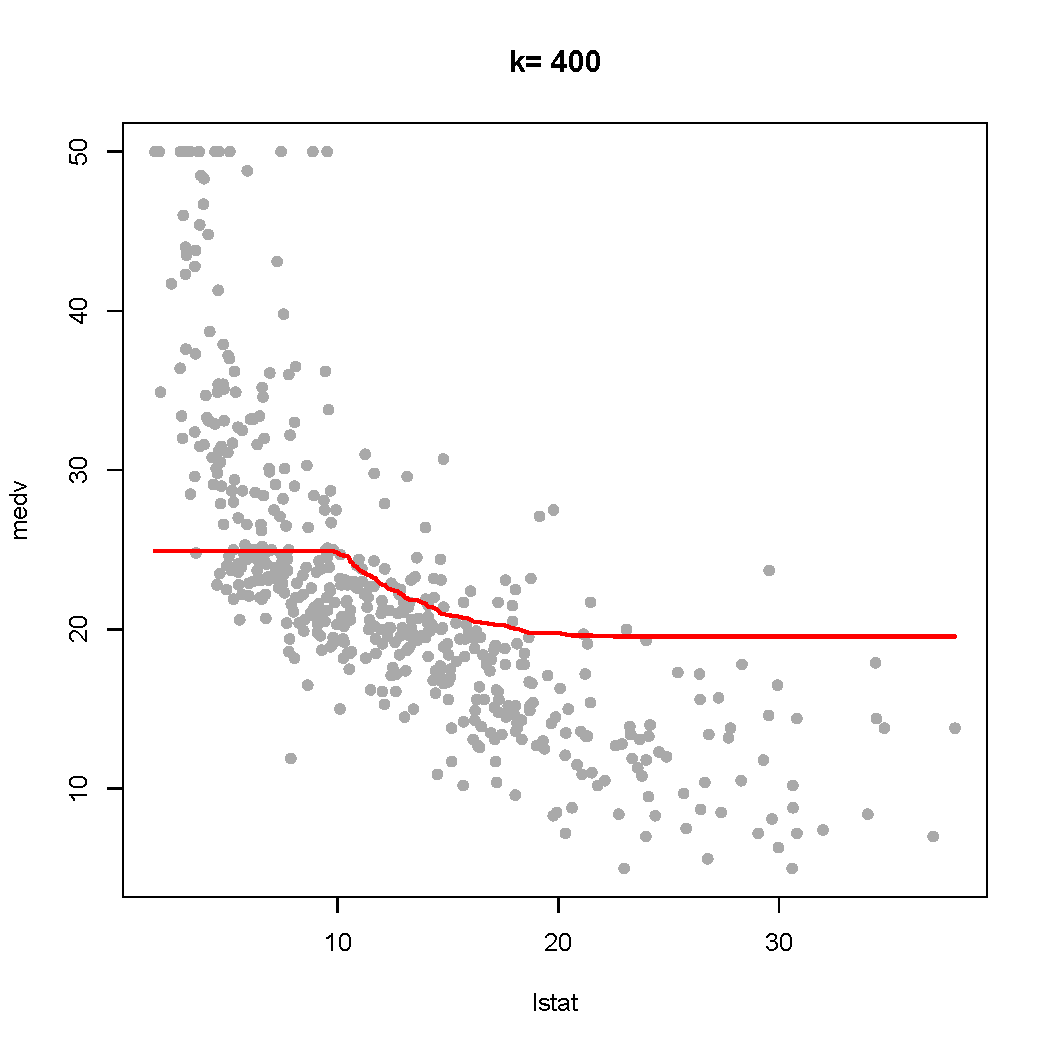
\includegraphics[width=3in]{k400}
\end{center}
\end{frame}

%%%%%%%%%%%%%%%%%%%%%%%%%%%%%%%
\begin{frame}
\frametitle{Back to Boston Housing}
{\color{blue}Okay, that seems sensible but why not use 5 neighbors or 200 neighbors? }

\vspace{-0.5cm}
\begin{center}
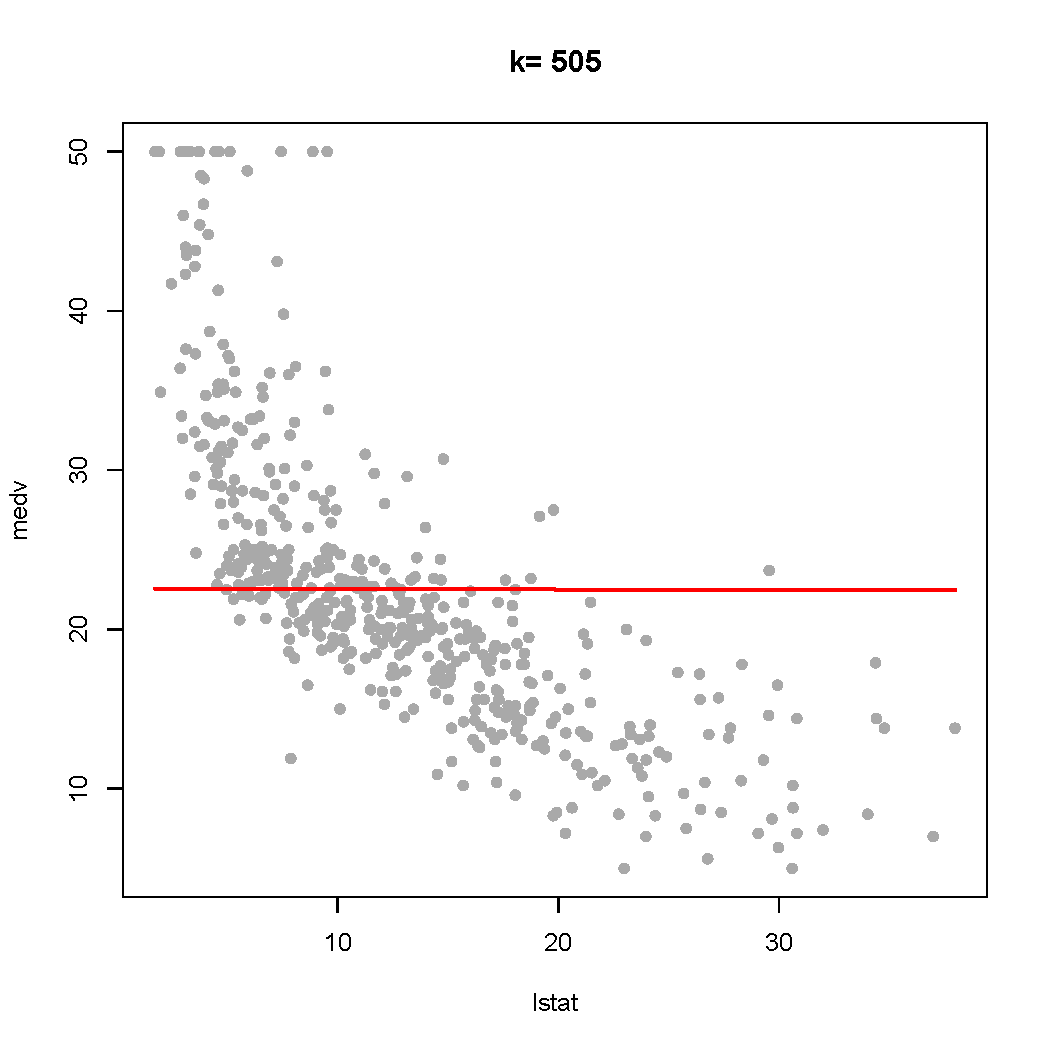
\includegraphics[width=3in]{k550}
\end{center}
\end{frame}


%%%%%%%%%%%%%%%%%%%%%%%%%%%%%%%
\begin{frame}
\frametitle{Complexity, Generalization and Interpretation}
\begin{itemize}
\item As we have seen in the examples above, there are lots of options in estimating $f(X)$. 
\item Some methods are very flexible some are not... {\color{red}{\it why would we ever choose a less flexible model?}}
\begin{enumerate}
\item Simple, more restrictive methods are usually easier to interpret 
\item More importantly, it is often the case that simpler models are {\color{blue}more accurate} in making future predictions.
\end{enumerate}
\end{itemize}


\vspace{-0.1cm}
\begin{center}
{\color{red}Not too simple, but not too complex!}
\end{center}

\vspace{-1cm}
\begin{center}
\begin{tabular}{ccc}
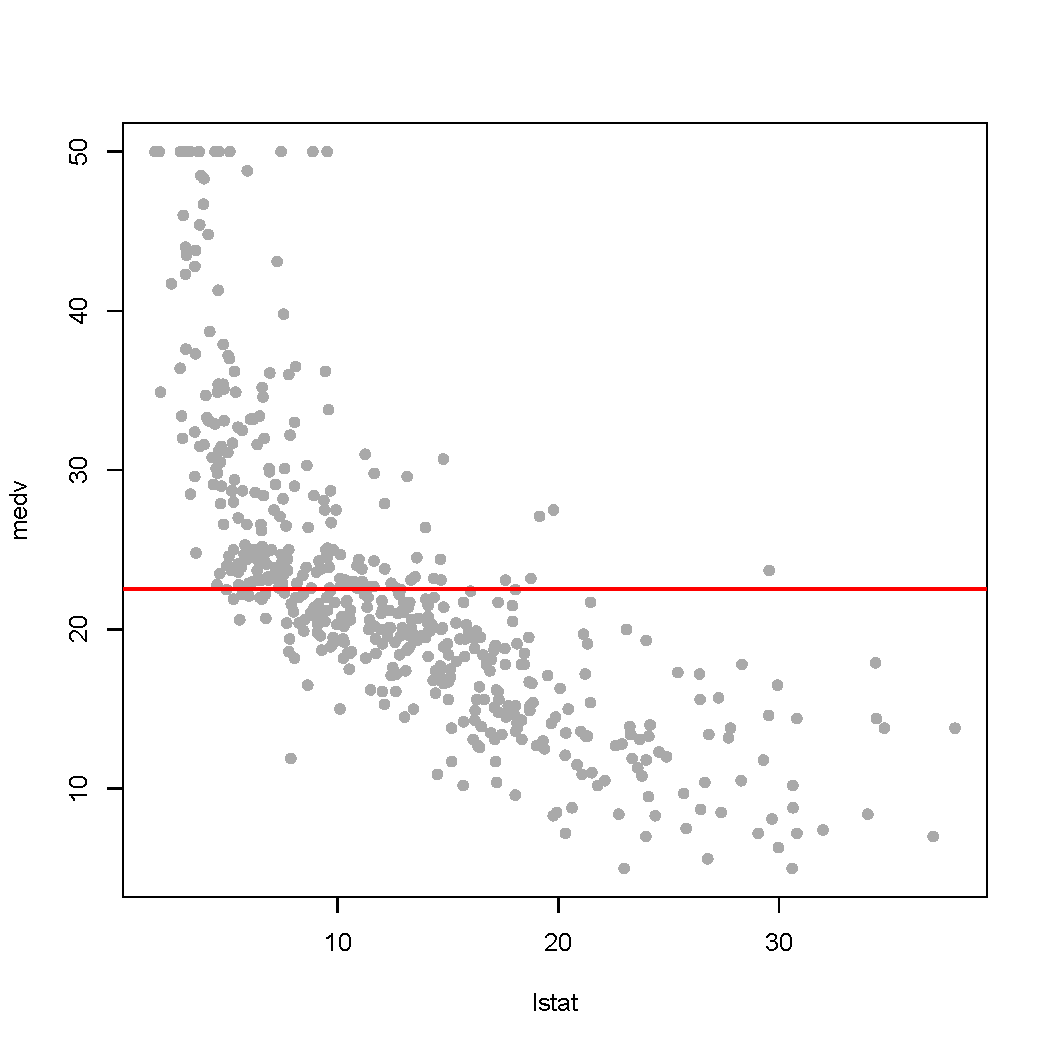
\includegraphics[width=1.4in]{Boston2}&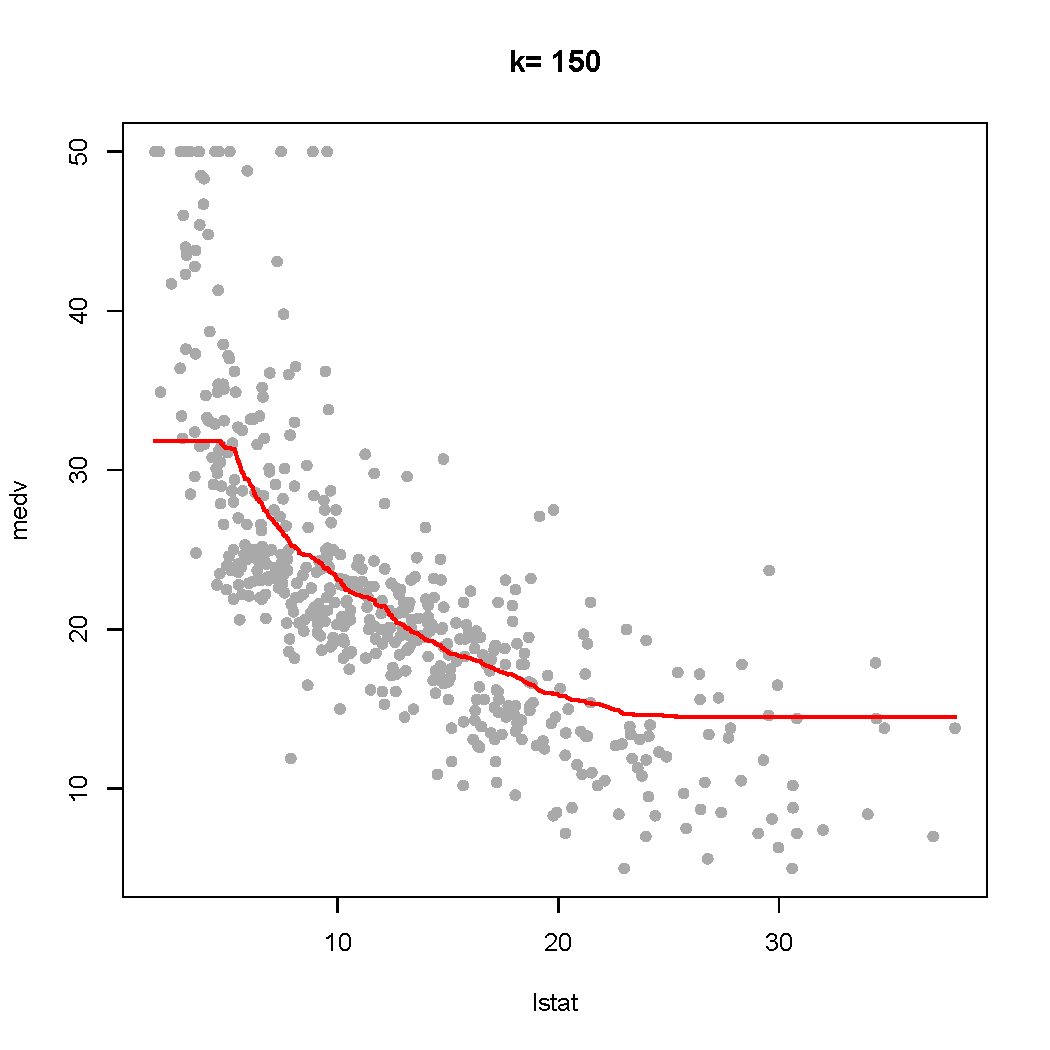
\includegraphics[width=1.4in]{k150}&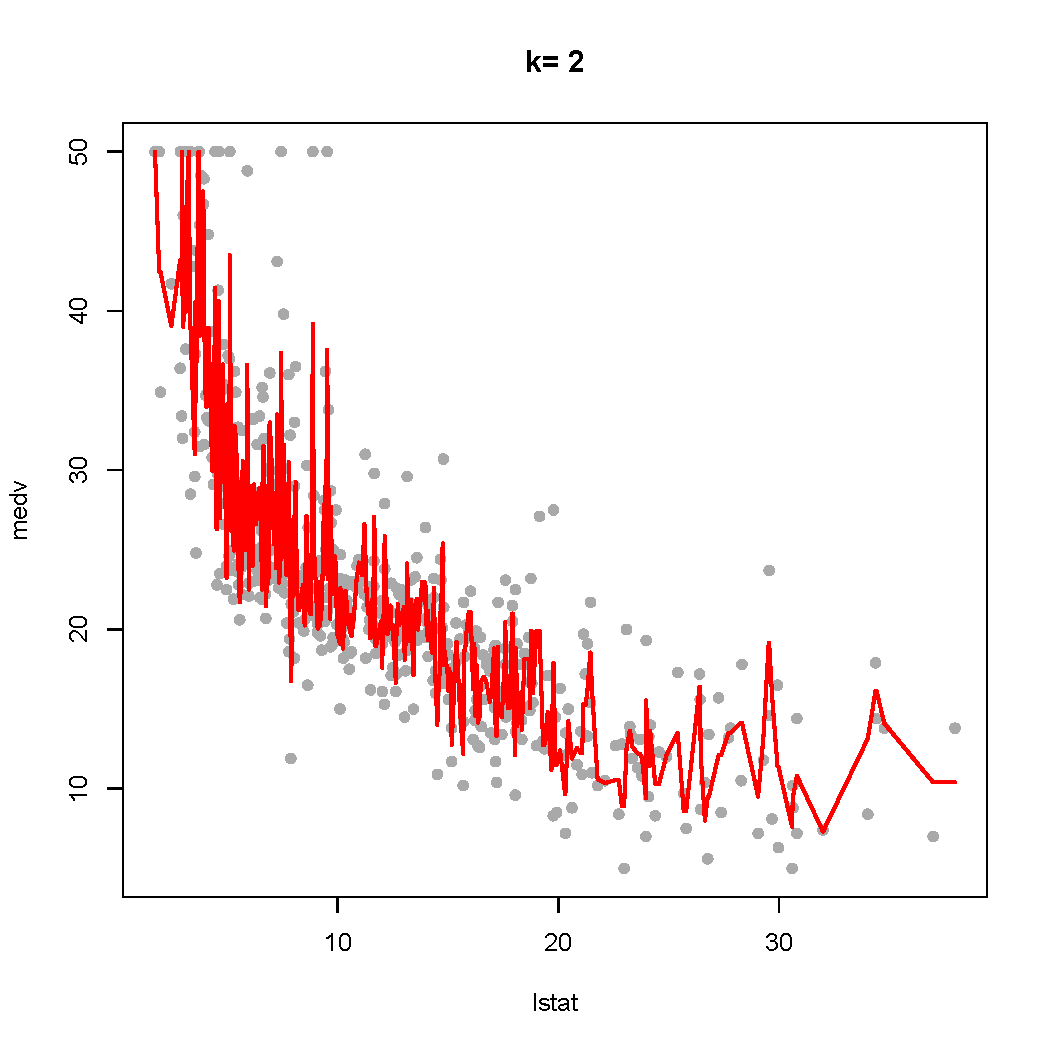
\includegraphics[width=1.4in]{k2}
\end{tabular}
\end{center}
\end{frame}



\section{\arabic{section}. Measuring Accuracy}
%%%%%%%%%%%%%%%%%%%%%%%%%%%%%%%
\begin{frame}
\frametitle{\arabic{section}. Measuring Accuracy}
{\color{red}How accurate are each of these models?}

\skoo 
Using the training data a standard measure of accuracy is the {\color{blue} \it root mean-squared error}
$$
RMSE = \sqrt{\frac{1}{n} \sum_{i=1}^n \left[Y_i - \widehat{f(X_i})\right]^2}
$$

\skoo 
This measure, on average, how large the ``mistakes'' (errors) made by the model are... 

\end{frame}

%%%%%%%%%%%%%%%%%%%%%%%%%%%%%%%
\begin{frame}
\frametitle{Measuring Accuracy (Boston housing, again)}
\vspace{-0.8cm}
\begin{center}
\begin{tabular}{ccc}
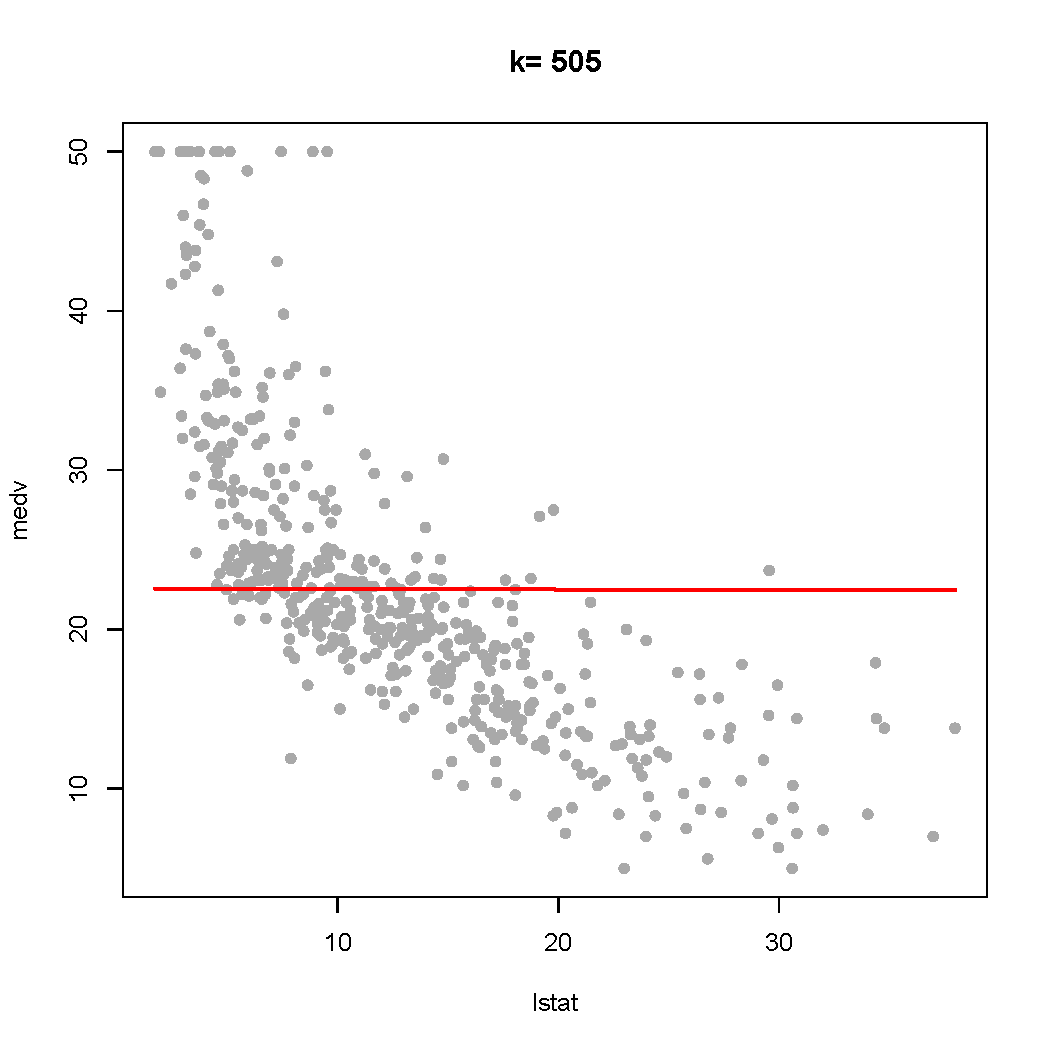
\includegraphics[width=1.4in]{k550}&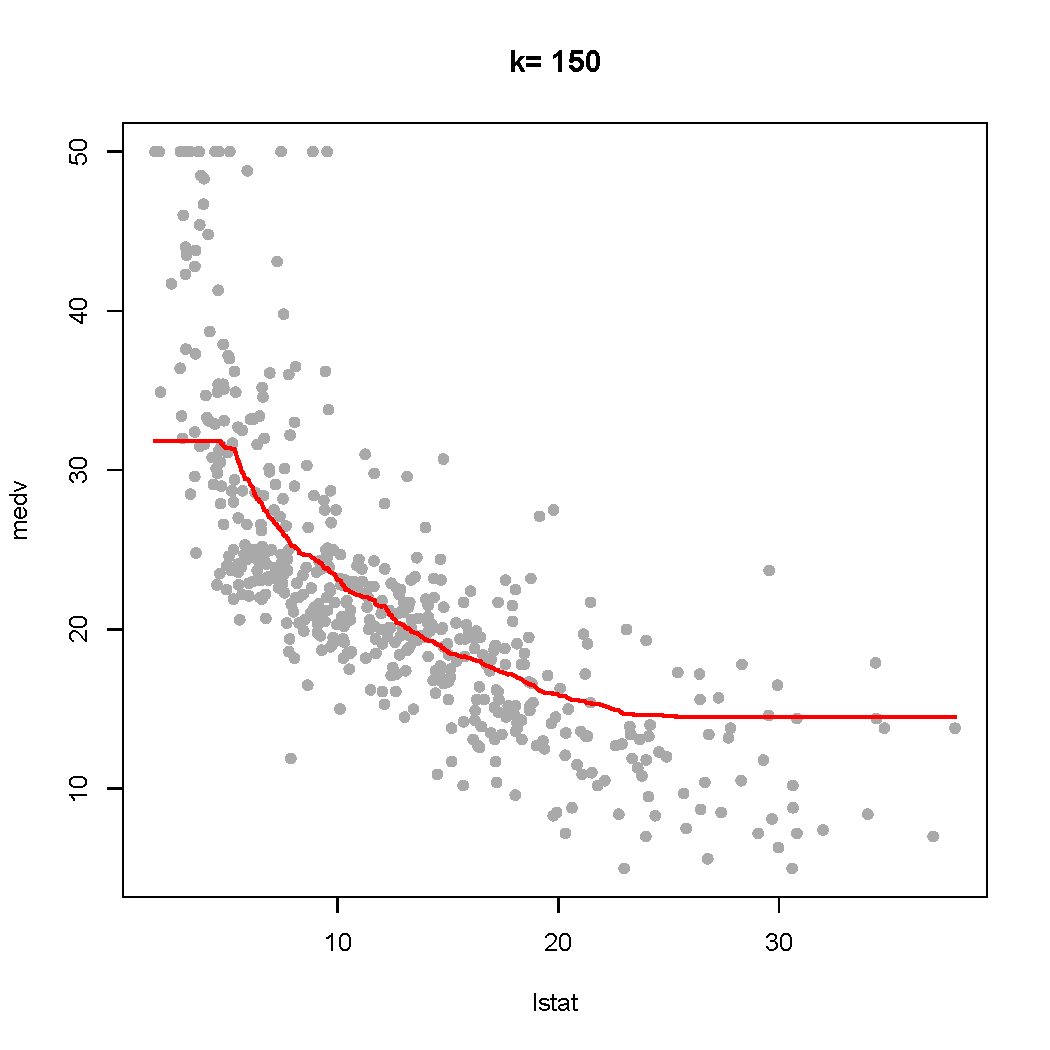
\includegraphics[width=1.4in]{k150}&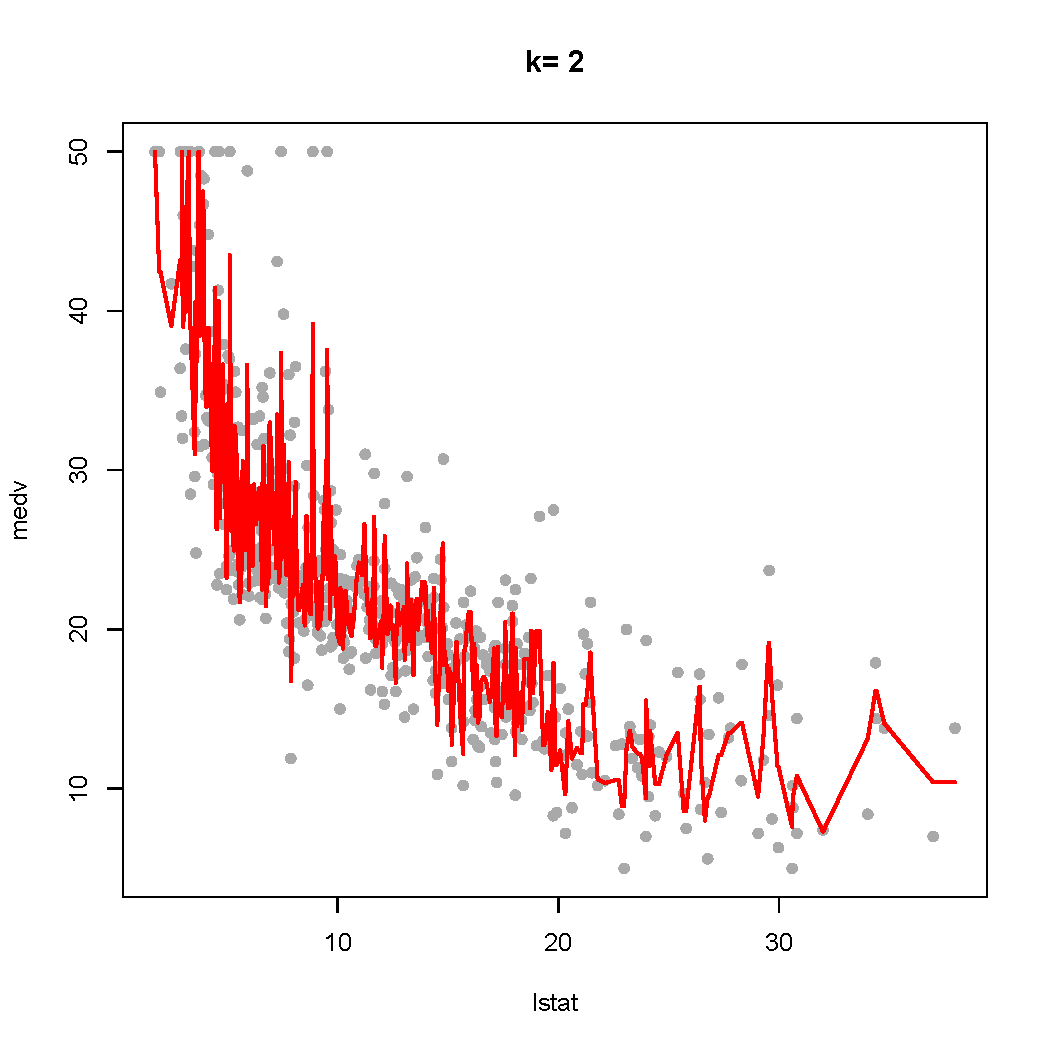
\includegraphics[width=1.4in]{k2}
\end{tabular}
\end{center}

\vspace{-1.2cm}
\begin{minipage}{2.1in}	
\begin{center}
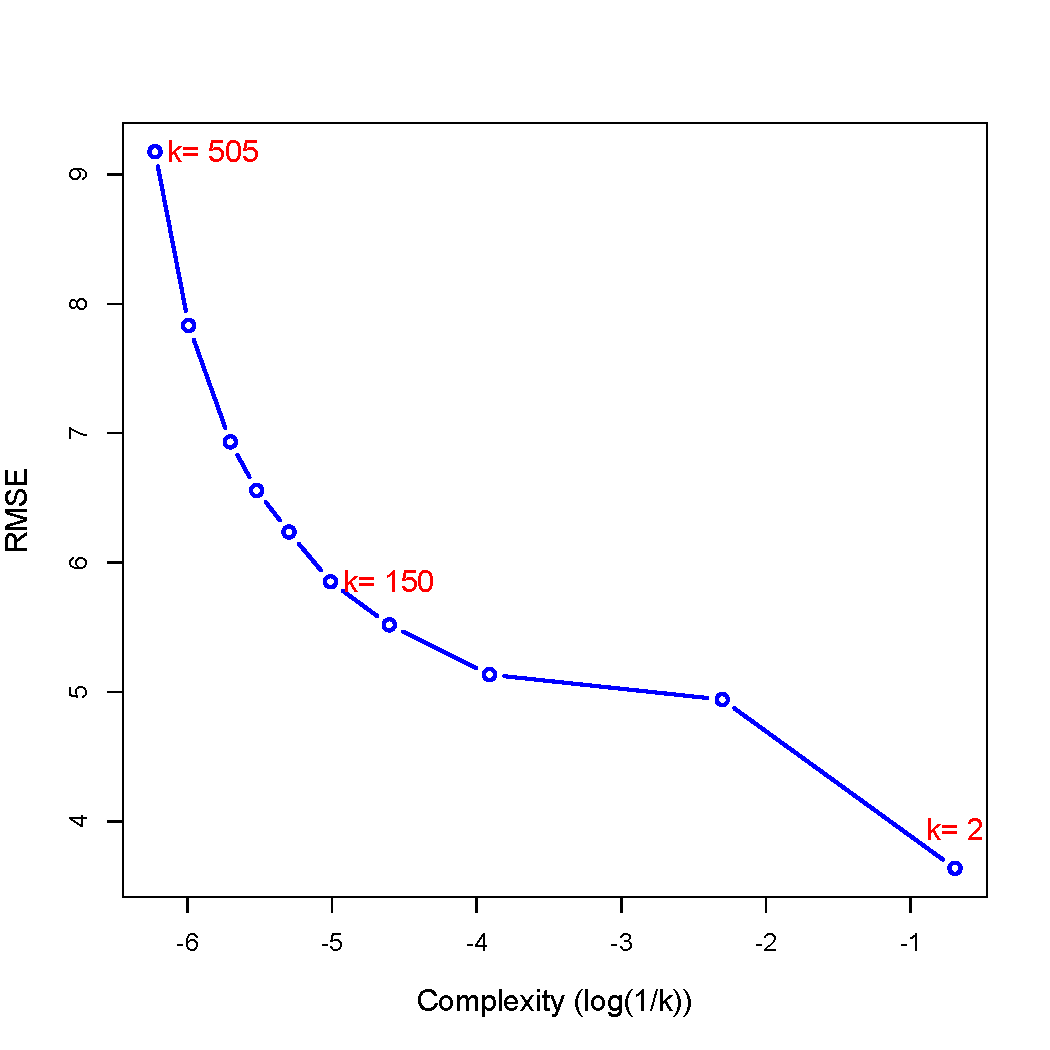
\includegraphics[width=2.2in]{BostonRMSE-0}
\end{center}
\end{minipage}
\begin{minipage}{2in}	
So, I guess we should just go with the most complex model, i.e., $k=2$, right?
\end{minipage}
\end{frame}


\section{\arabic{section}. Out-of Sample Predictions}
%%%%%%%%%%%%%%%%%%%%%%%%%%%%%%%
\begin{frame}
\frametitle{\arabic{section}. Out-of Sample Predictions}
But, do we really care about explaining what we have already seen?

\skoo

{\color{blue}Key Idea:} what really matters is our prediction accuracy {\color{red}out-of-sample!!!}

\skoo
Suppose we have $m$ additional observations $(X^o_i,Y^o_i)$, for $i=1,\dots,m$, {\color{blue}that we did not use to fit the model.} Let's call this dataset the {\color{red}{\it validation set} }(also known as {\it hold-out set} or {\it test set}) 

\skoo
Let's look at the out-of-sample RMSE:
$$
RMSE^o = \sqrt{\frac{1}{m} \sum_{i=1}^m \left[Y^o_i - \widehat{f(X^o_i})\right]^2}
$$

\end{frame}


%%%%%%%%%%%%%%%%%%%%%%%%%%%%%%%
\begin{frame}
\frametitle{Out-of Sample Predictions}
In our Boston housing example, I randomly chose a training set of size 400. I re-estimate the models using only this set and use the models to predict the remaining 106 observations (validation set)...

\vspace{-0.3cm}
\begin{minipage}{2.5in}
\begin{center}
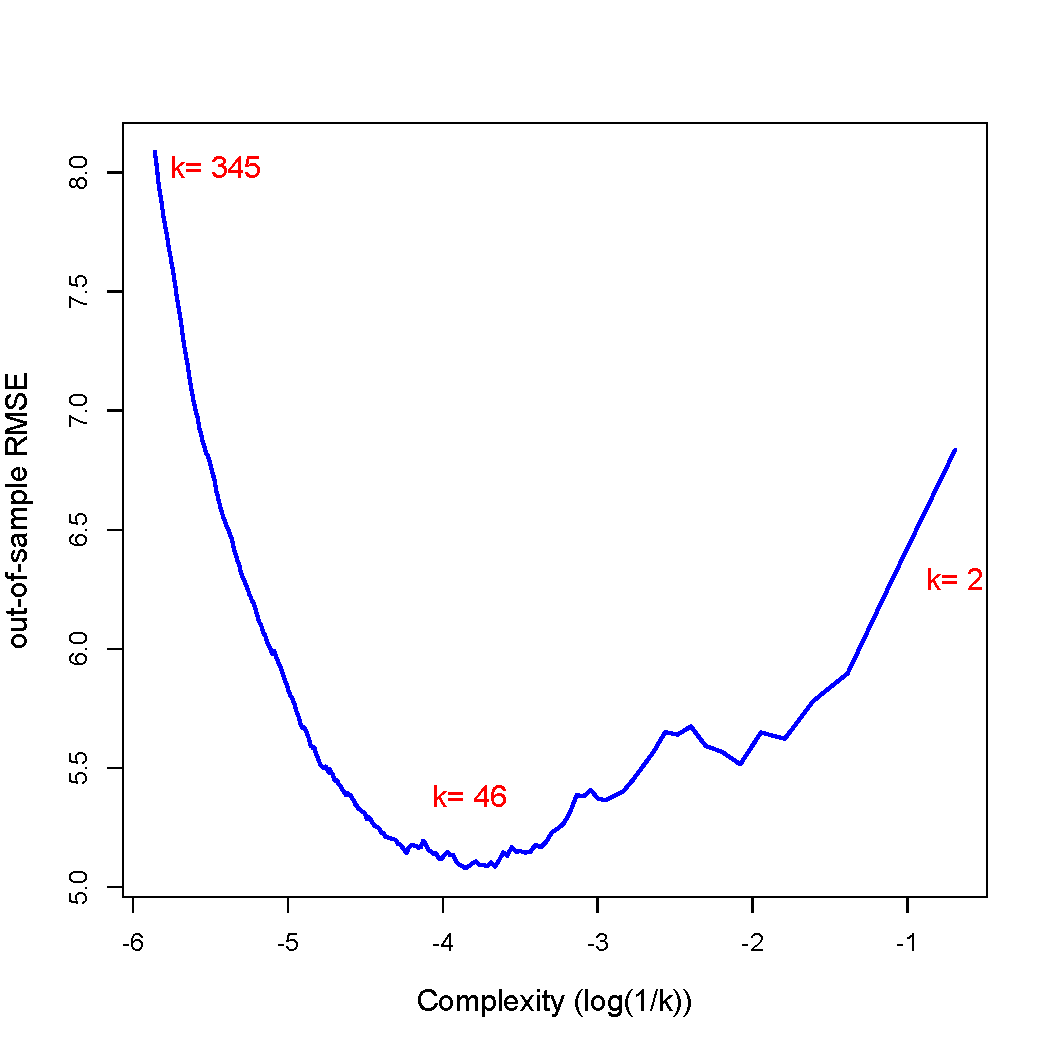
\includegraphics[width=2.6in]{BostonRMSE_OOS}
\end{center}
\end{minipage}
\begin{minipage}{1.5in}

{\color{blue}\it Now, the model where $k=46$ looks like the most accurate choice!!}

\sko

{\color{red}Not too simple but not too complex!!!}
\end{minipage}

\end{frame}

%%%%%%%%%%%%%%%%%%%%%%%%%%%%%%%
\begin{frame}
\frametitle{The Key Idea of the Course!!}

\vspace{-0.8cm}
\begin{center}
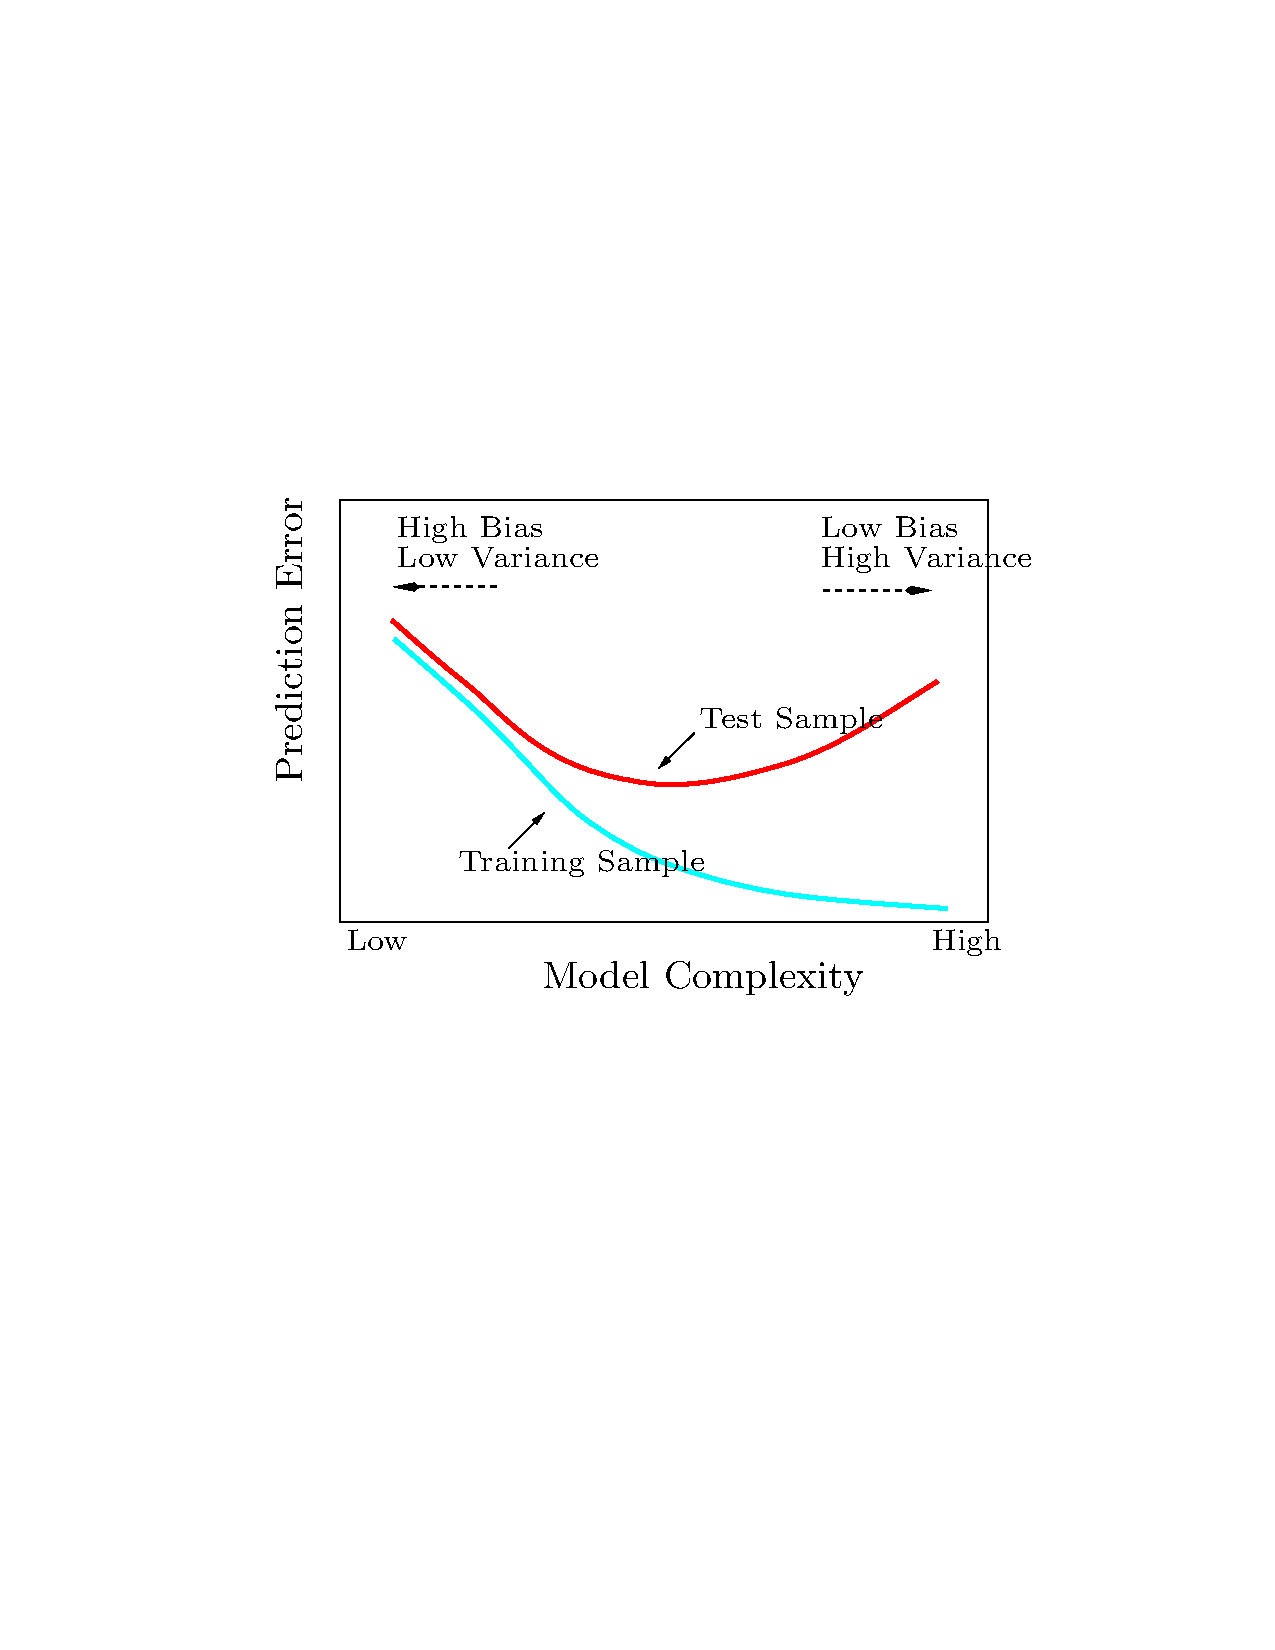
\includegraphics[width=3in]{ESL_2-11}
\end{center}

\vspace{-0.2cm}
This shows the typical behavior of the in and out-of-sample prediction error as a function of the complexity of the model... too flexible models will adapt itself too closely to the the training set and will not generalize well, i.e., not be very good for the test data.
\end{frame}


\section{\arabic{section}. Bias-Variance Trade-Off}
%%%%%%%%%%%%%%%%%%%%%%%%%%%%%%%
\begin{frame}
\frametitle{\arabic{section}. Bias-Variance Trade-Off}
{\color{red}
Why do complex models behave poorly in making predictions?  
}

\skoo
Let's start with an example...

\begin{itemize}
\item In the Boston housing example, I will randomly choose 30 observations to be in the training set 3 different times... 
\item for each training set I will estimate $f(\cdot)$ using the $k$-nearest neighbors idea...  first with $k=2$ and them with $k=20$
\end{itemize}

\end{frame}

%%%%%%%%%%%%%%%%%%%%%%%%%%%%%%%
\begin{frame}
\frametitle{Bias-Variance Trade-Off}
{\color{red} k=2}  Hi variability...
\begin{center}
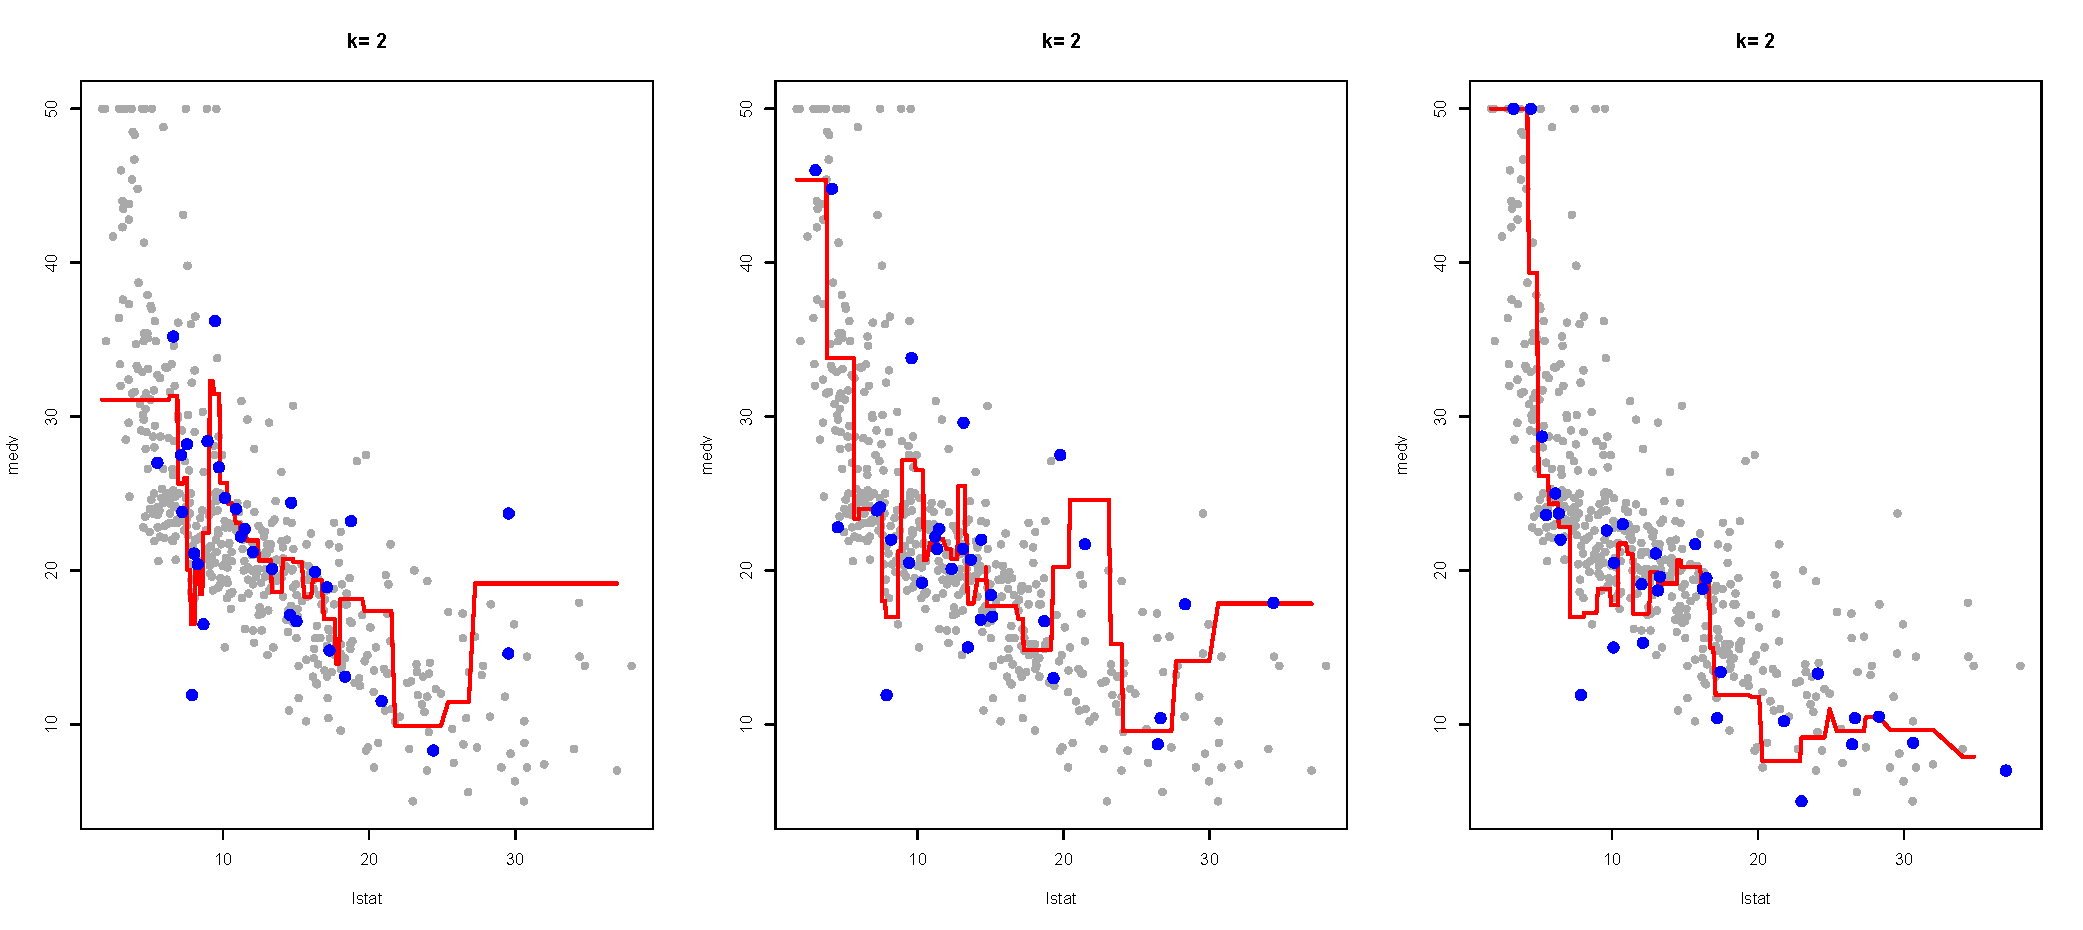
\includegraphics[width=4.5in]{knn2VAR}
\end{center}
({\color{blue}blue points} are the training data used)
\end{frame}

%%%%%%%%%%%%%%%%%%%%%%%%%%%%%%%
\begin{frame}
\frametitle{Bias-Variance Trade-Off}
{\color{red} k=20} Low variability ... but BIAS!!
\begin{center}
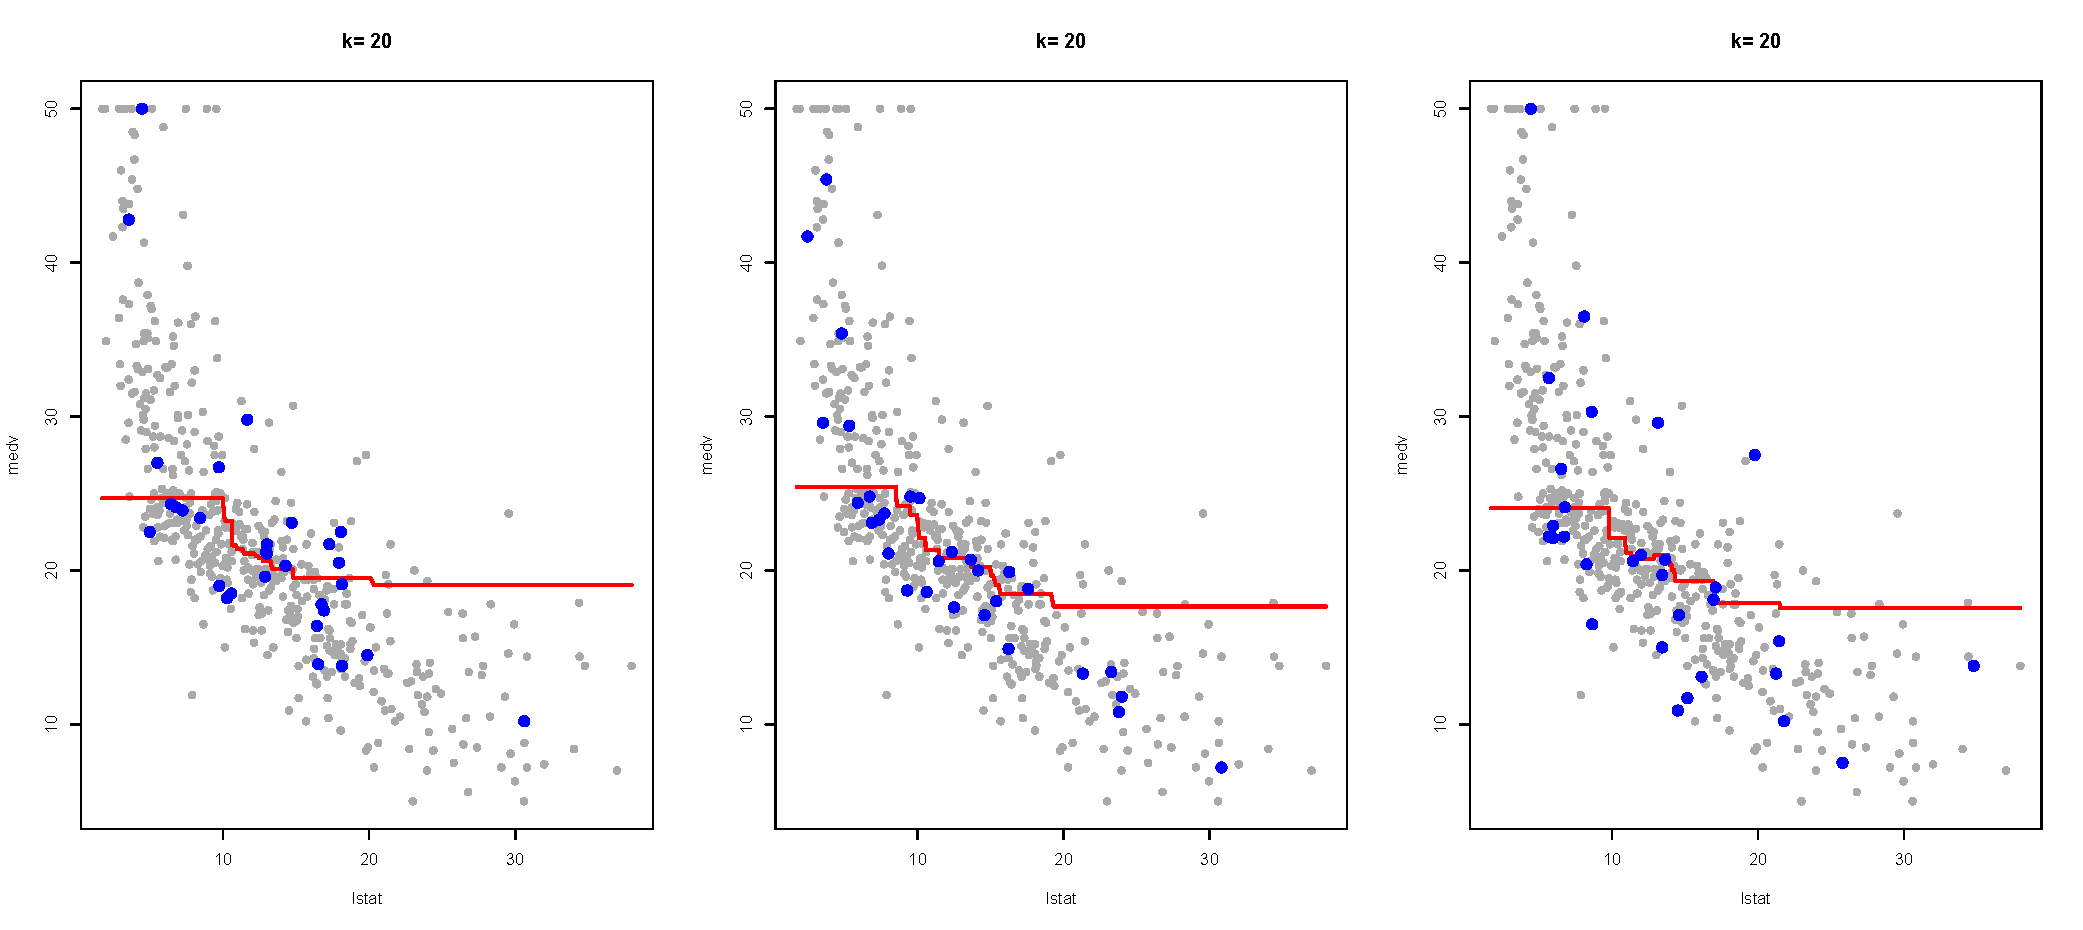
\includegraphics[width=4.5in]{knn20VAR}
\end{center}
({\color{blue}blue points} are the training data used)
\end{frame}

%%%%%%%%%%%%%%%%%%%%%%%%%%%%%%%
\begin{frame}
\frametitle{Bias-Variance Trade-Off}
{\color{blue}What did we see here?}

\begin{itemize}
\item When $k=2$, it seems that the estimate of $f(\cdot)$ varies a lot between training sets...
\item When $k=20$ the estimates look a lot more stable...
\end{itemize}

\skoo

{\color{red}
Now, imagine that you are trying to predict $medv$ when $lstat=20$... compare the changes in the predictions made by the different training sets under $k=2$ and $k=20$... what do you see? 
}
\end{frame}


%%%%%%%%%%%%%%%%%%%%%%%%%%%%%%%
\begin{frame}
\frametitle{Bias-Variance Trade-Off}
\begin{itemize}
\item This is an illustration of what is called the {\color{blue}\it bias-variance trade-off}. 
\item In general, simple models are trying to explain a complex, real problem with not a lot of flexibility so it introduces {\color{blue}bias}...
on the other hand, by being simple the estimates tend to have low {\color{red}variance}
\item On the other hand, complex models are able to quickly adapt to the real situation and hence lead to small {\color{blue}bias}... however, by being to adaptable, it tends to vary a lot, i.e., high {\color{red}variance}.
\end{itemize}
\end{frame}

%%%%%%%%%%%%%%%%%%%%%%%%%%%%%%%
\begin{frame}
\frametitle{Bias-Variance Trade-Off}
\begin{itemize}
\item In other words, we are trying to capture important patterns of the data that {\color{blue}generalize} to the future observations we are trying to predict. Models that are too simple are not able to capture relevant patterns and might have too big of a bias in predictions...
\item Models that are too complex will ``chase'' irrelevant patterns in the training data that are not likely to exist in future data... so, it will lead to predictions that will vary a lot as things could change a lot depending on what sample we happen to see.
\item {\color{red}Our goal is to find the sweet spot in the bias-variance trade-off!!}
\end{itemize}
\end{frame}

%%%%%%%%%%%%%%%%%%%%%%%%%%%%%%%
\begin{frame}
\frametitle{Bias-Variance Trade-Off}

Once again, this is the key idea of the course!!

\vspace{-0.1cm}
\begin{center}
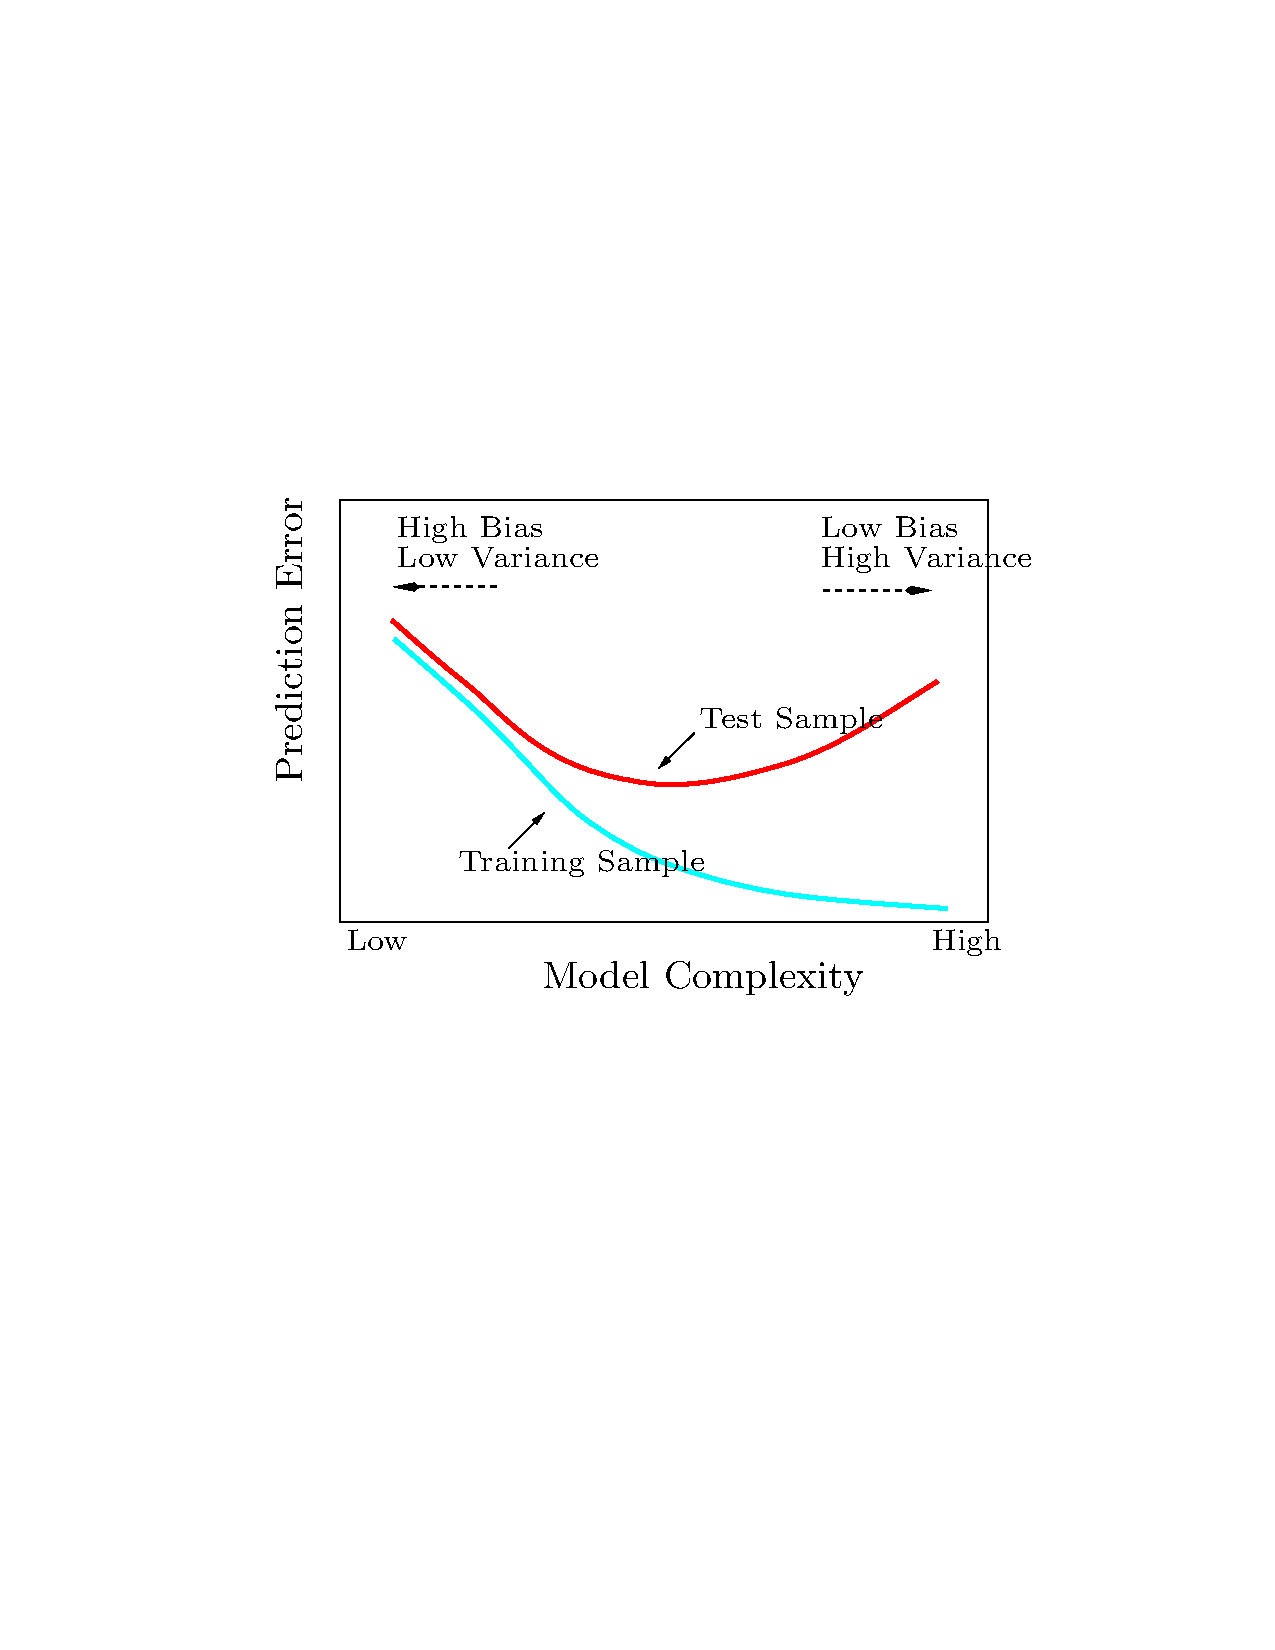
\includegraphics[width=3in]{ESL_2-11}
\end{center}

\end{frame}



%%%%%%%%%%%%%%%%%%%%%%%%%%%%%%%
\begin{frame}
\frametitle{Bias-Variance Trade-Off}

Let's get back to our original representation of the problem... it helps us understand what is going on...
$$
Y_f = f(X_f) + \epsilon
$$
\begin{itemize}
\item We need flexible enough models to find $f(\cdot)$ without imposing bias...
\item ... but, too flexible models will ``chase'' non-existing patterns in $\epsilon$ leading to unwanted variability
\end{itemize}

\end{frame}


%%%%%%%%%%%%%%%%%%%%%%%%%%%%%%%
\begin{frame}
\frametitle{Bias-Variance Trade-Off}
A more detailed look at this idea... assume we are trying to make a prediction for $Y_f$ using $X_f$ and our inferred $\widehat{f(\cdot)}$. We hope to make small mistake measured by squared distance... Let's explore how our mistakes will behave {\color{red}\it on average}.

\begin{eqnarray*}
\mbox{E}\left[ (Y_f - \widehat{f(X_f)})^2\right] &=& {\color{blue}\left(f(X_f) - \mbox{E}\left[\widehat{f(X_f)}\right] \right)^2} +  {\color{red}\mbox{Var}\left[ \widehat{f(X_f)}\right]} + \mbox{Var}(\epsilon) \\
&=&  {\color{blue}\mbox{Bias}\left[\widehat{f(X_f)}\right]^2} +  {\color{red}\mbox{Var}\left[ \widehat{f(X_f)}\right]} +\mbox{Var}(\epsilon)
\end{eqnarray*}

\sko

hence, the {\it Bias-Variance Trade-Off!!}


\end{frame}



\section{\arabic{section}. Classification}
%%%%%%%%%%%%%%%%%%%%%%%%%%%%%%%
\begin{frame}
\frametitle{\arabic{section}. Classification}
{\color{red}Classification} is the term used when we want to predict a $Y$ that is a category... win/lose, sick/healthy, pay/default, good/bad... below is an example where we are trying to predict whether or not the favorite team will win as a function of the Vegas' betting point-spread. 

\begin{center}
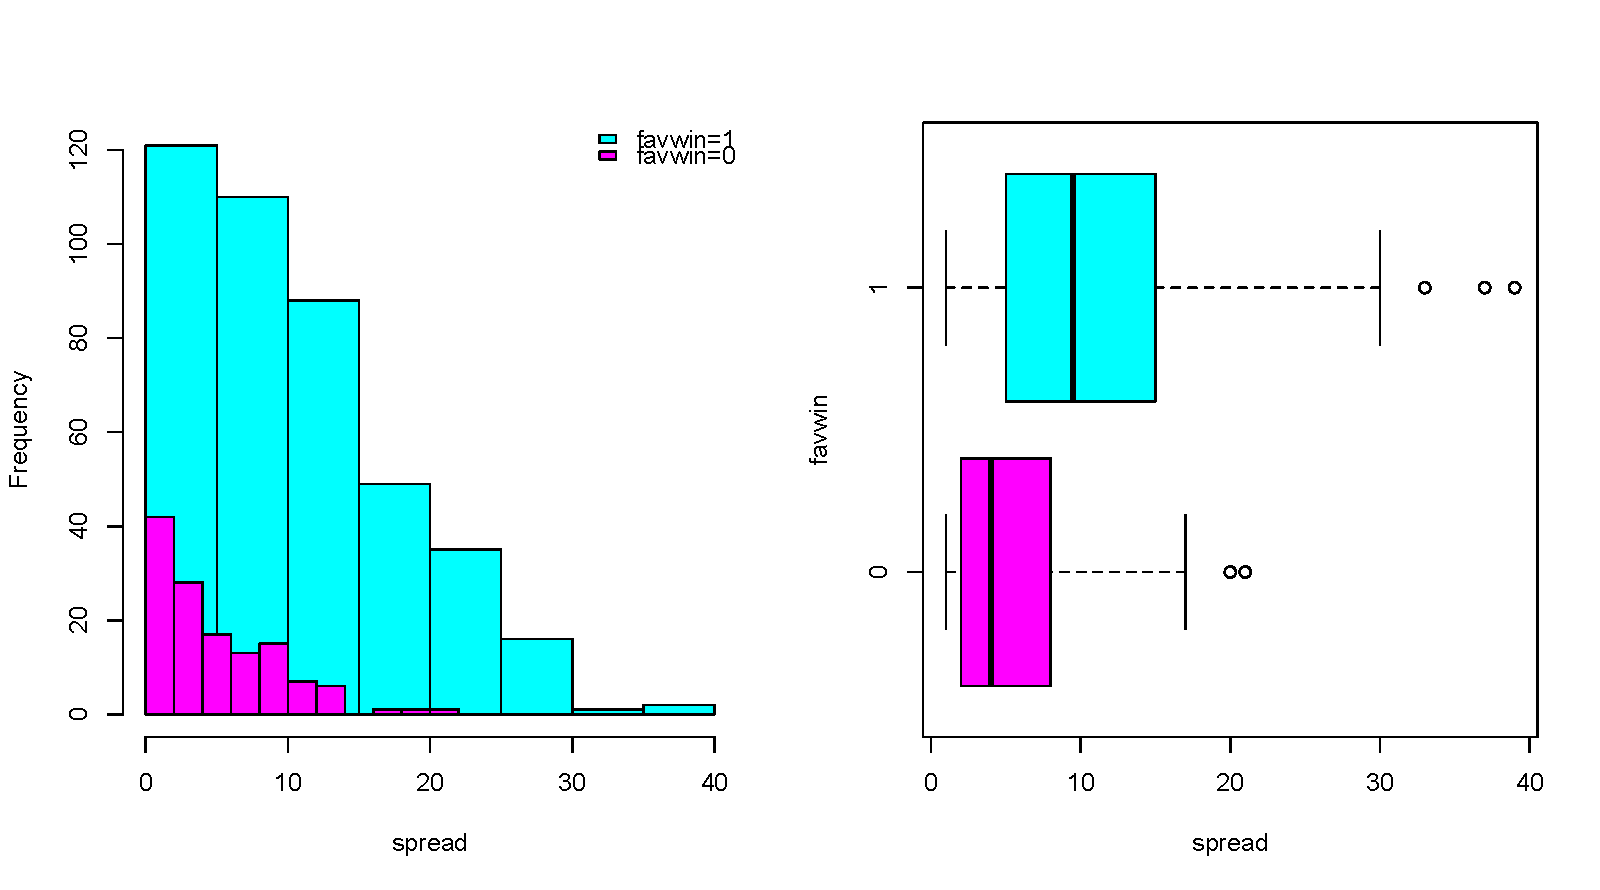
\includegraphics[width=3.5in]{NBA1}
\end{center}
\end{frame}


%%%%%%%%%%%%%%%%%%%%%%%%%%%%%%%
\begin{frame}
\frametitle{Classification}
In this context, $f(X)$ will output the {\color{blue}probability} of $Y$ taking a particular category (win/lose,here). Below, the black line represent different methods to estimate $f(X)$ in this example.

\vspace{-0.3cm}
\begin{center}
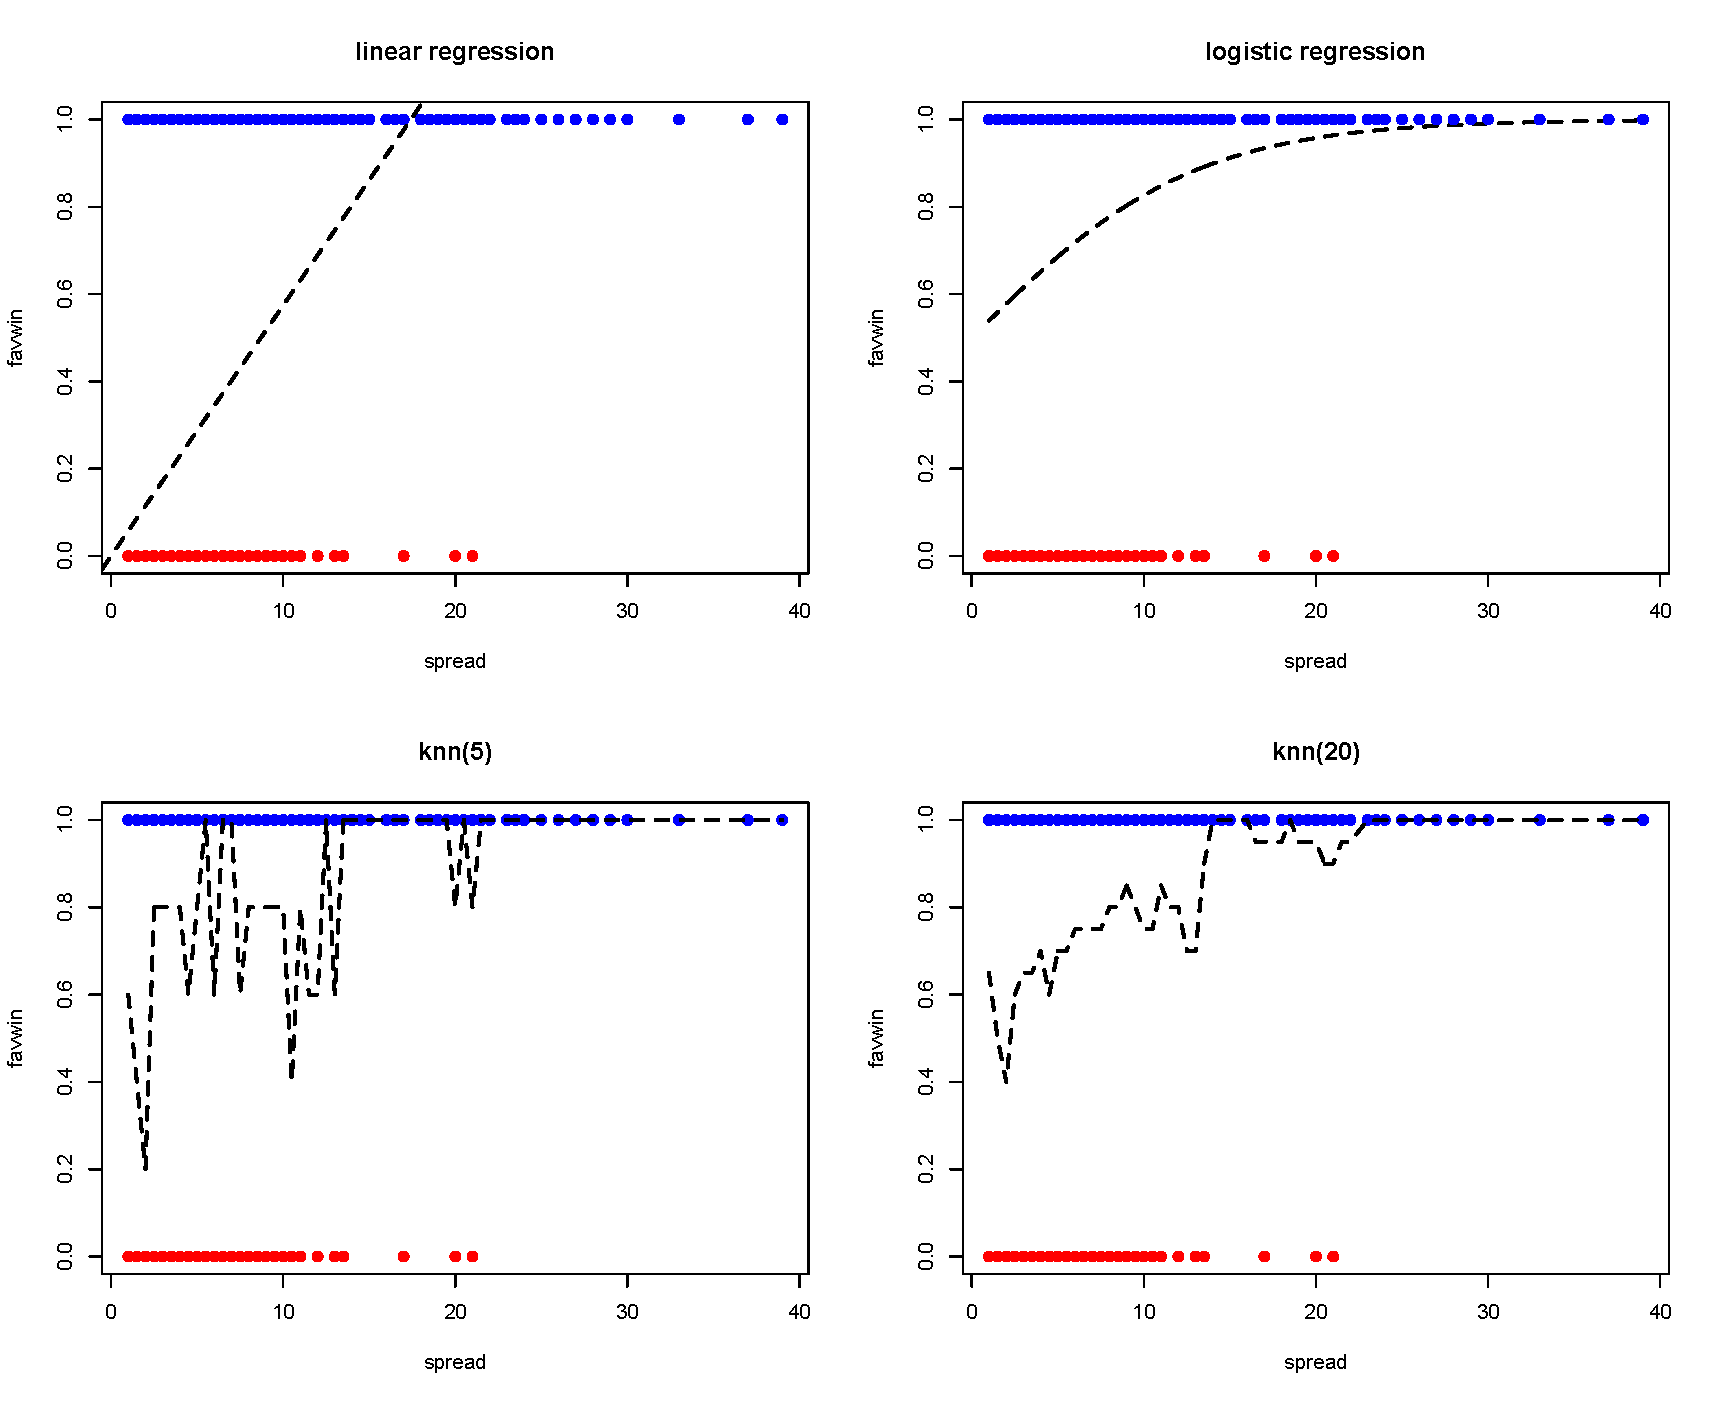
\includegraphics[width=3.3in]{NBAModels}
\end{center}
\end{frame}

%%%%%%%%%%%%%%%%%%%%%%%%%%%%%%%
\begin{frame}
\frametitle{Classification}
All the discussion about complexity vs. predictive accuracy (bias-variance trade-off) applies to this setting... what differs is our measure of accuracy as we are no longer dealing with a numerical outcome variable. A common approach is to measure the {\color{red} \it error rate}, i.e., the number of times we a estimated $\widehat{f(\cdot)}$ ``gets it wrong''... in the training set (with $n$ observations) define the error rate as:
$$
\frac{1}{n} \sum_{i=1}^n \mbox{I}(Y_i \neq \hat{Y}_i)
$$
where $\hat{Y}_i$ is the class (category)  label assigned by $\widehat{f(X_i)}$ and $\mbox{I}(\cdot)$ is an indicator variable that equals 1 whenever $Y_i \neq \hat{Y}_i$ and 0 otherwise. 
\end{frame}


%%%%%%%%%%%%%%%%%%%%%%%%%%%%%%%
\begin{frame}
\frametitle{Classification}

As mentioned above, in classification, $\widehat{f(X_i)}$ outputs a probability. In order to use this information and create a {\color{red}\it classification rule} we need to decide on a {\color{blue}cut-off} (or cut-offs) to determined the label assignments. 

\skoo

In general, if we are looking at only two categories (like the NBA example above) the standard cut-off is 0.5. This means that if  $\widehat{f(X_f)}>0.5$ we define $\hat{Y}_i=1$ ($\hat{Y}_i=0$ otherwise).

\skoo

Later on, we will think more carefully about defining cut-offs... 

\end{frame}


%%%%%%%%%%%%%%%%%%%%%%%%%%%%%%%
\begin{frame}
\frametitle{Classification}
\begin{itemize}
\item Extending this metric to the testing set is straightforward. For $m$ samples  $(X^o_i,Y^o_i)$ the error rate is:
$
\frac{1}{m} \sum_{i=1}^n \mbox{I}(Y^o_i \neq \hat{Y}^o_i)
$
\item In general, we need to think carefully about choosing the cut-off and defining a classification rule. In the NBA example above, what is a natural cut-off? 
\item The error rate treats a {\color{red}``mistake''} equally, regardless of its type. Is that always a good idea? Think about deciding if a defender is guilty or not? 
\item We will explore all of these issues more carefully when we get to the classification section. For now, let's keep the error rate as our accuracy measure.
\end{itemize}

\end{frame}

\section{\arabic{section}. Cross-Validation}
%%%%%%%%%%%%%%%%%%%%%%%%%%%%%%%
\begin{frame}
\frametitle{\arabic{section}. Cross-Validation}
\begin{itemize}
\item Using a {\color{blue}validation-set} to evaluate the performance of competing models has two potential drawbacks: 
\begin{enumerate}
\item the results can be highly dependent on the choice of the validation set... what samples? how many?
\item by leaving aside a subset of data for validation we end up estimating the models with less information. It is harder to {\it learn} with fewer samples and this might lead to an overestimation of errors.  
\end{enumerate}
\item {\color{blue} Cross-Validation} is a refinement of the validation strategy that help address both of these issues.
\end{itemize}

\end{frame}




%%%%%%%%%%%%%%%%%%%%%%%%%%%%%%%
\begin{frame}
\frametitle{Leave-One-Out Cross-Validation (loocv)}

The name says it all! 
\begin{itemize}
\item Assume we have $n$ samples in our dataset. Define the validation set by choosing only {\color{red}one sample}. Call it the $i^{th}$ observation...
\item The model is then trained in the remaining $n-1$ samples and the results are used to predict the left-out sample. Compute the squared-error $MSE_i = (Y_i - \hat{Y}_i)^2$
\item {\color{red}Repeat the procedure for every sample in the dataset ($n$ times) and compute the average cross-validation MSE:
$$
MSE^{loocv} = \frac{1}{n}\sum_{i=1}^n MSE_i
$$}
\end{itemize}
\end{frame}



%%%%%%%%%%%%%%%%%%%%%%%%%%%%%%%
\begin{frame}
\frametitle{Leave-One-Out Cross-Validation}
In the Boston data.... 
\vspace{-1cm}
\begin{center}
\begin{tabular}{cc}
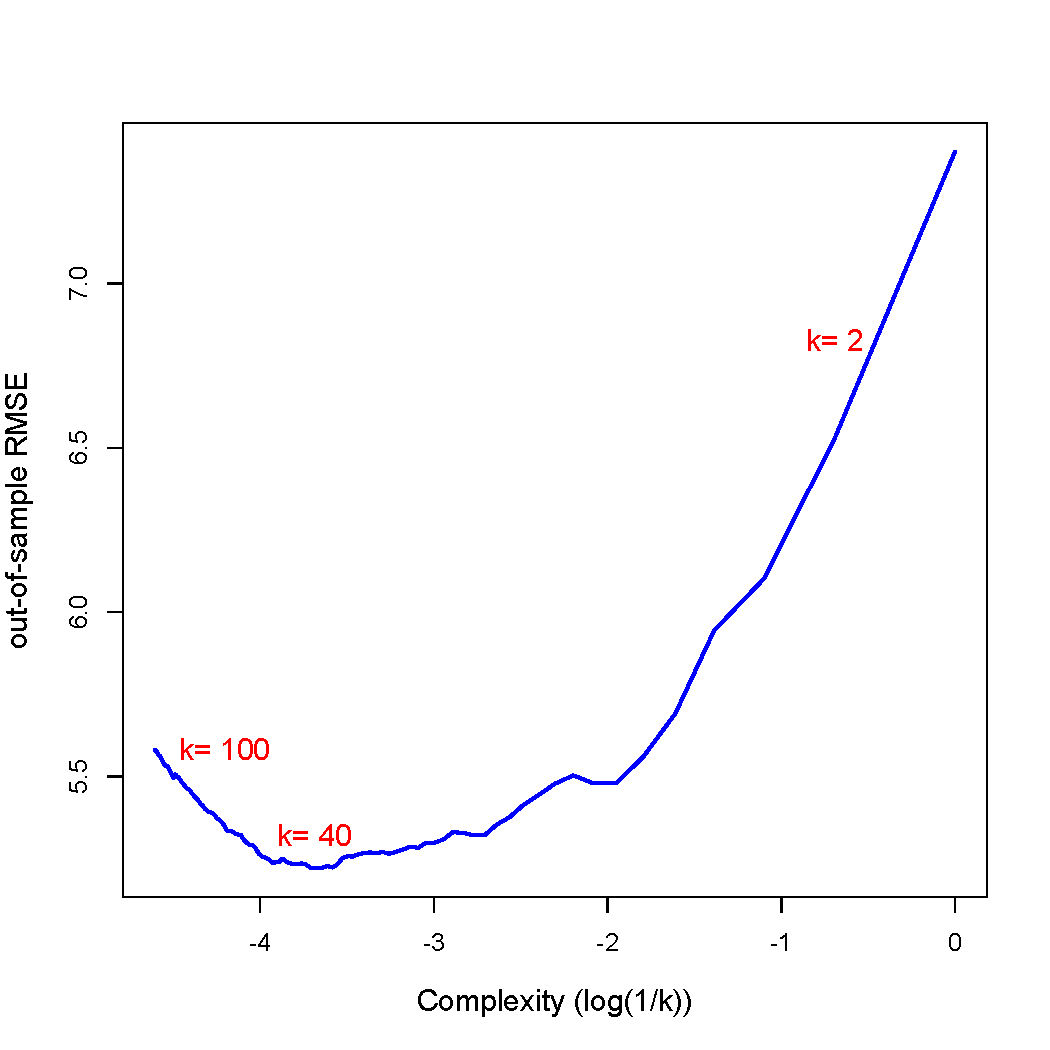
\includegraphics[width=2.2in]{Boston_LOOCV}&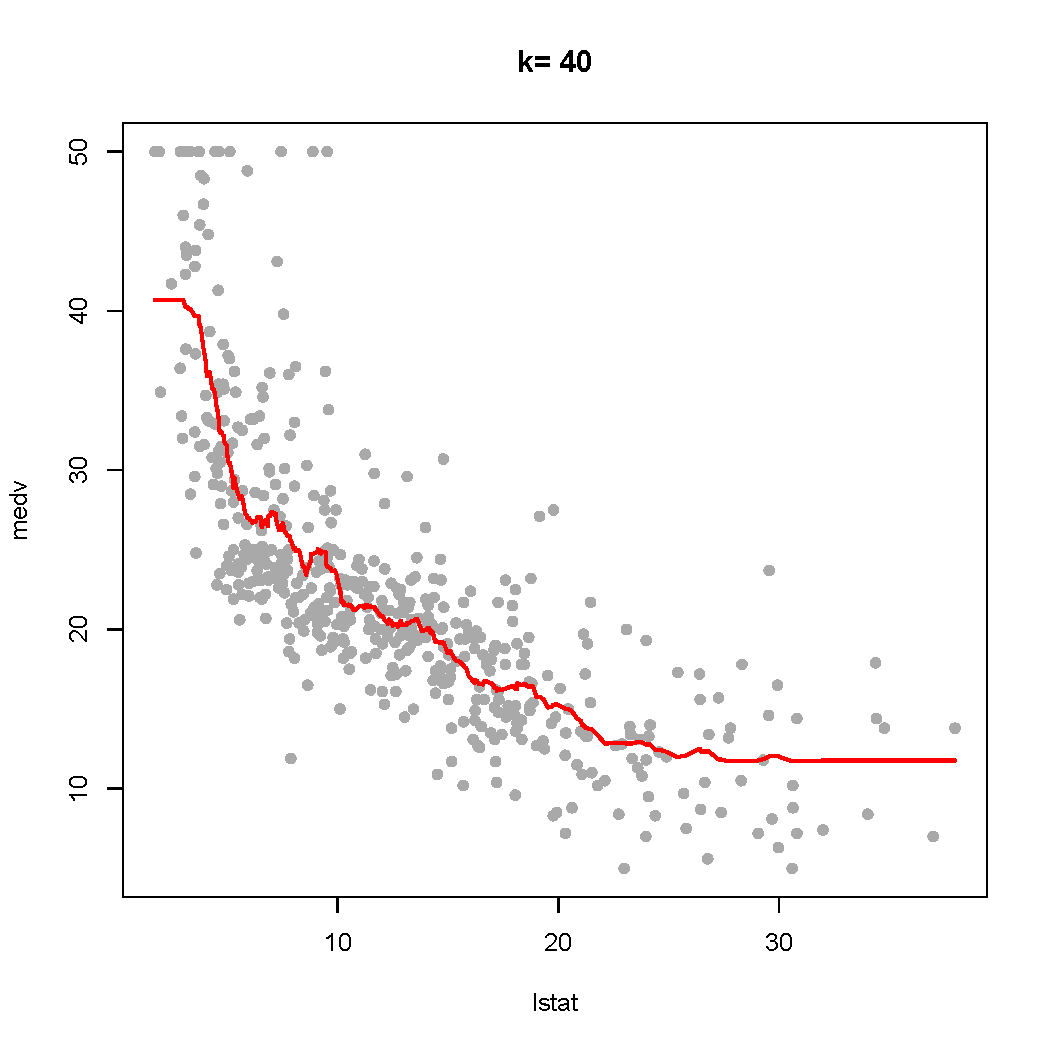
\includegraphics[width=2.2in]{Bostonk40}\\
\end{tabular}
\end{center}

\end{frame}

%%%%%%%%%%%%%%%%%%%%%%%%%%%%%%%


\begin{frame}
\frametitle{$k$-fold Cross Validation}

LOOCV can be computationally expensive as each model being considered has to be estimated $n$ times! A popular alternative is what is called {\color{blue}$k$-fold Cross Validation.}

\begin{itemize}
\item This approach randomly divides the original dataset into {\color{blue}$k$ groups} of approximately the same size
\item Choose one of the groups as a validation set. Estimate the models with the remaining $k-1$ groups and predict the samples in the validation set. Compute the average squared-error for the samples in the validation set $MSE_i = \mbox{Average}\left[(Y_i - \hat{Y}_i)^2\right]$ 
\item {\color{red}Repeat the procedure for every $fold$ in the dataset ($k$ times) and compute the average cross-validation MSE:
$
MSE^{kcv} = \frac{1}{k}\sum_{i=1}^k MSE_i
$}
\end{itemize}
\end{frame}



%%%%%%%%%%%%%%%%%%%%%%%%%%%%%%%
\begin{frame}
\frametitle{$k$-fold Cross Validation}
{\color{blue}The usual choices are between $k=5$ and $k=10$...}
\begin{center}
\begin{tabular}{cc}
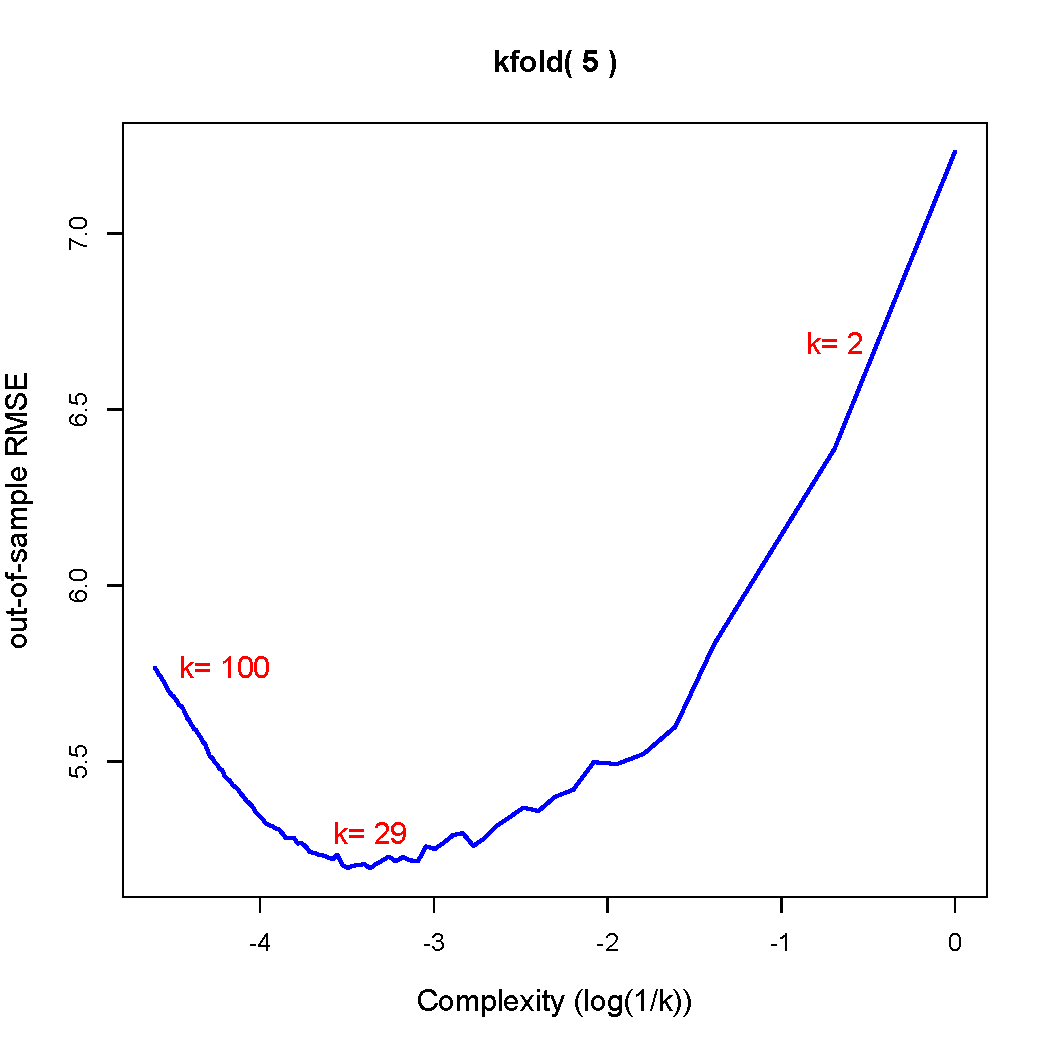
\includegraphics[width=2.2in]{Boston_kfold5}&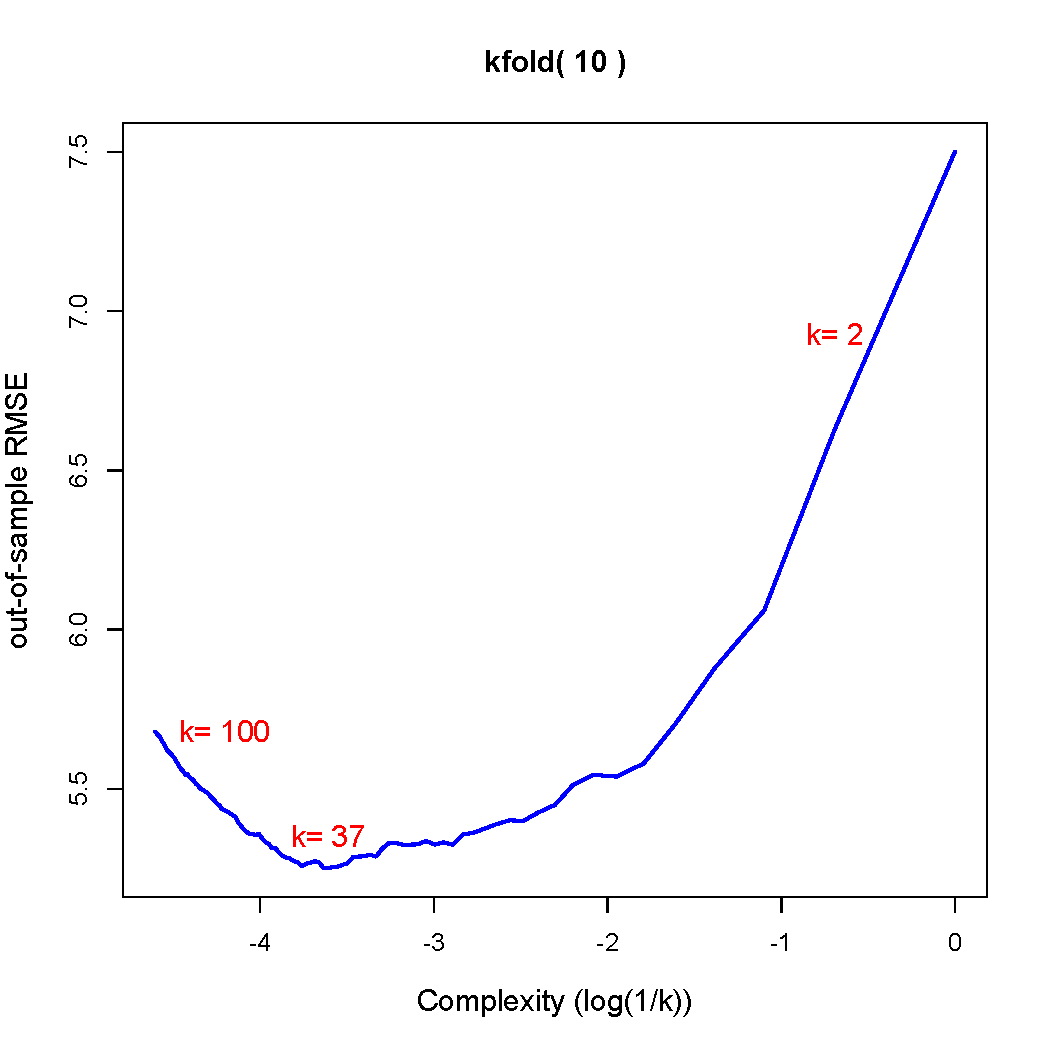
\includegraphics[width=2.2in]{Boston_kfold10}\\
\end{tabular}
\end{center}
\end{frame}

%%%%%%%%%%%%%%%%%%%%%%%%%%%%%%%
\begin{frame}
\frametitle{$k$-fold Cross Validation}
\begin{itemize}
\item {\color{blue} Bias-Variance Trade-Off:} LOOCV has a smaller bias as it uses more information in the training sets... but it also has more variance! By only leaving a sample out at a time, the training set doesn't change much so the outputs will be very correlated with each other. So, the resulting MSE will be a average off correlated quantities which tends to be more variable
\item In $k$-fold the outputs are not very correlated as the training sets can be quite different and the resulting MSE is an average of somewhat ``independent'' quantities... hence less variance! 
\item {\color{red}There is a bias-variance trade-off between LOOCV and $k$-fold. The choice of $k=5$ or $k=10$ has been empirically shown to be a good choice that neither suffers from a lot of bias nor from a lot of variance!}
\end{itemize}
\end{frame}




\section{\arabic{section}. $k$-Nearest Neighbors (kNN)}
%%%%%%%%%%%%%%%%%%%%%%%%%%%%%%%
\begin{frame}
\frametitle{\arabic{section}. $k$-Nearest Neighbors (kNN)}

The {\color{blue}$k$-nearest neighbors} algorithm will try to {\it predict} (numerical variables) or {\it classify} (categorical variables) based on {\color{blue}similar (close) records} on the {\it training dataset}. 

\skoo

Remember, the problem is to guess a future value $Y_f$ given new values of  the covariates $X_f = (x_{1f}, x_{2f}, x_{3f}, \dots, x_{pf})$.

\end{frame}

%%%%%%%%%%%%%%%%%%%%%%%%%%%%%%%
\begin{frame}
\frametitle{$k$-Nearest Neighbors (kNN)}

{\bf {\color{blue} kNN:} How do the $Y's$ look like close to the region around $X_f$?} \\ We need to find the {\color{red}$k$} records in the training dataset that are close to $X_f$. How? ``Nearness'' to the $i^{th}$ neighbor can be defined by (euclidian distance):
$$
d_i = \sqrt{\sum_{j=1}^p (x_{jf} - x_{ji})^2}
$$

\sko

{\bf Prediction:}
\begin{itemize}
\item Numerical $Y_f$: take the average of the $Y's$ in the $k$-nearest neighbors
\item Categorical $Y_f$: take the most common category in the $k$-nearest neighbors 
\end{itemize}


\end{frame}

%%%%%%%%%%%%%%%%%%%%%%%%%%%%%%%
\begin{frame}
\frametitle{$k$-Nearest Neighbors (kNN) -- Example}

\vspace{-0.5cm}

\begin{center}
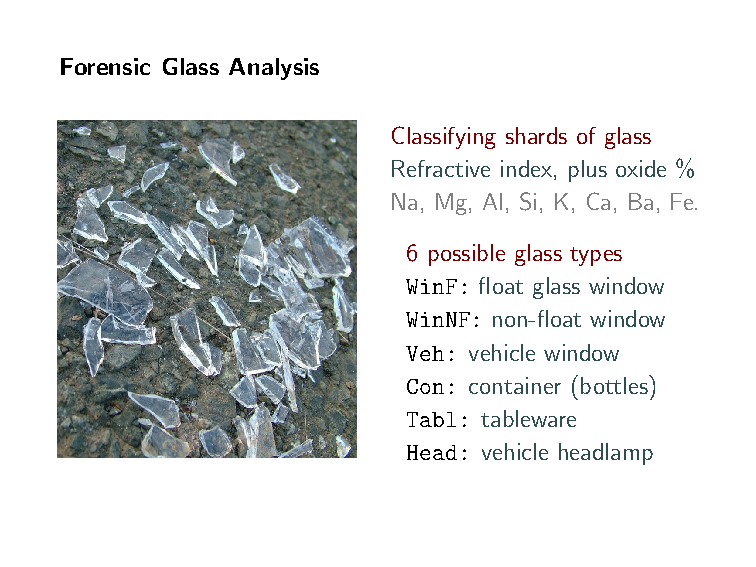
\includegraphics{glass0}
\end{center}

\end{frame}

%%%%%%%%%%%%%%%%%%%%%%%%%%%%%%%
\begin{frame}
\frametitle{$k$-Nearest Neighbors (kNN) -- Example}

\vspace{-0.7cm}

\begin{center}
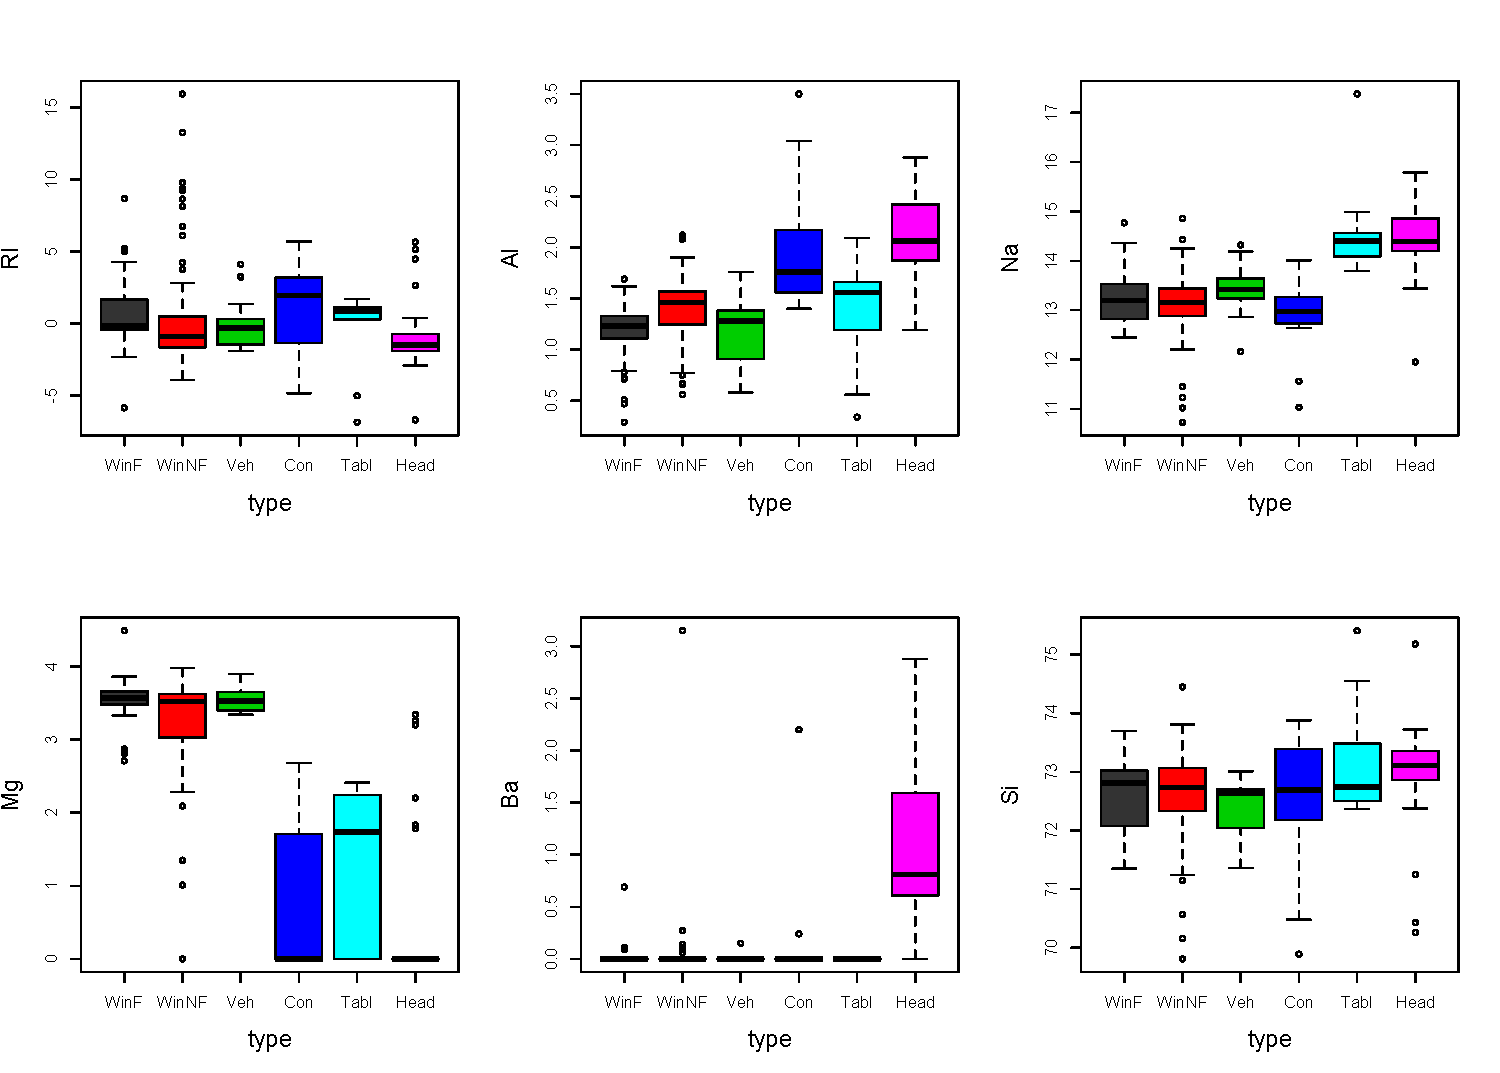
\includegraphics[width=4in]{glass1}
\end{center}

\vspace{-0.3cm}
Some variables are clear discriminators {\color{blue}(Ba)} while others are more subtle {\color{red}(RI)}
\end{frame}


%%%%%%%%%%%%%%%%%%%%%%%%%%%%%%%
\begin{frame}
\frametitle{$k$-Nearest Neighbors (kNN) -- Example}

Using only RI and AI let's try to predict the point marked by ``?''
\vspace{-0.5cm} 

\begin{center}
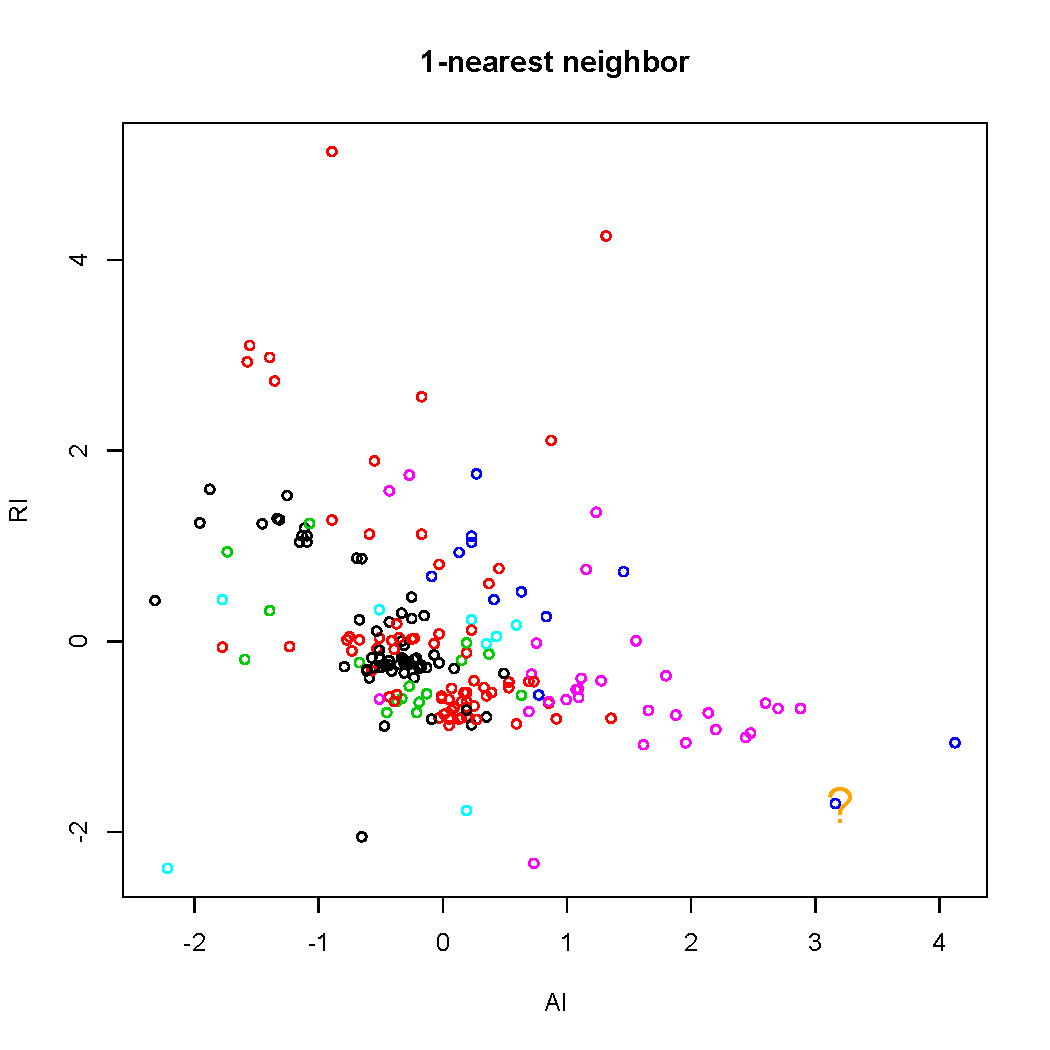
\includegraphics[width=3.3in]{knn1}
\end{center}

\end{frame}

%%%%%%%%%%%%%%%%%%%%%%%%%%%%%%%
\begin{frame}
\frametitle{$k$-Nearest Neighbors (kNN) -- Example}

\vspace{-0.5cm}

\begin{center}
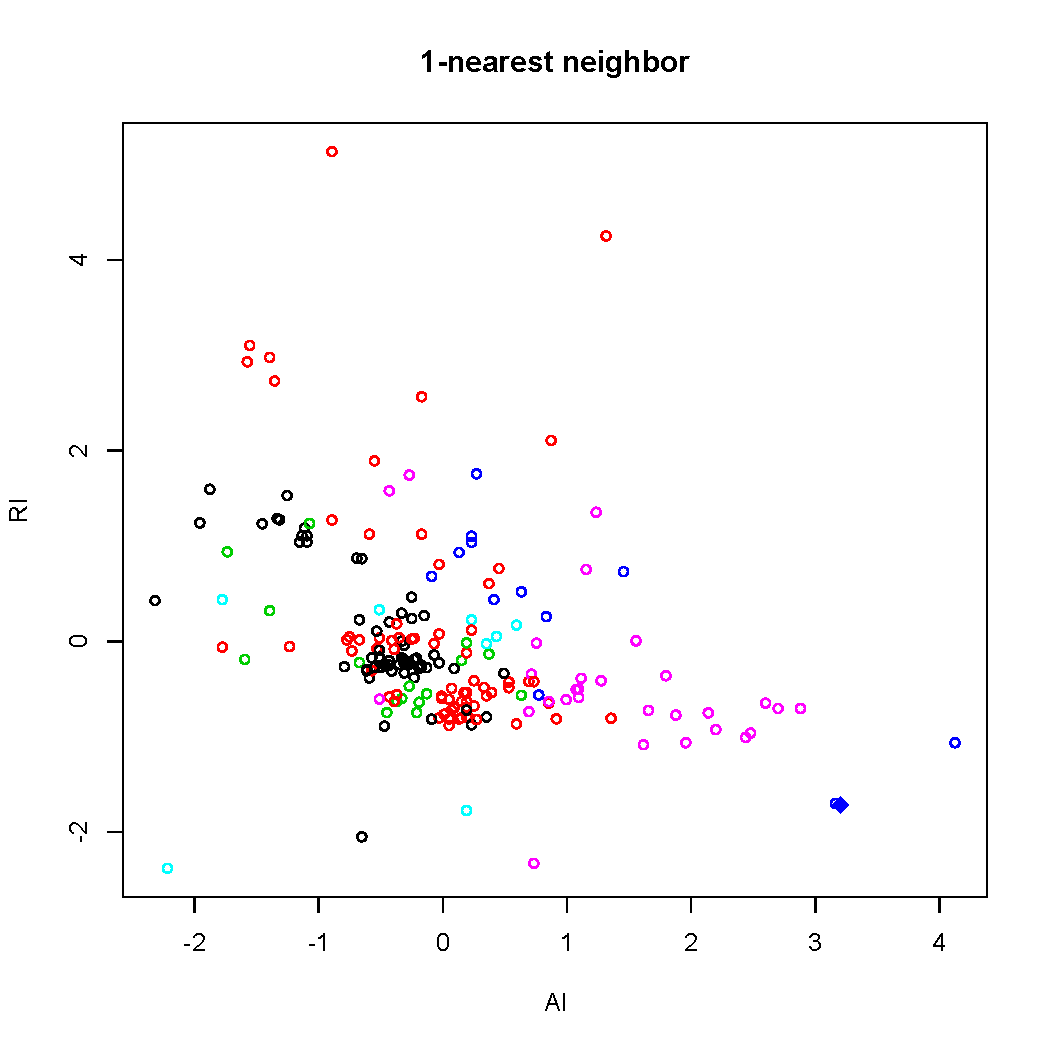
\includegraphics[width=3.4in]{knn2}
\end{center}

\end{frame}

%%%%%%%%%%%%%%%%%%%%%%%%%%%%%%%
\begin{frame}
\frametitle{$k$-Nearest Neighbors (kNN) -- Example}

\vspace{-0.5cm}

\begin{center}
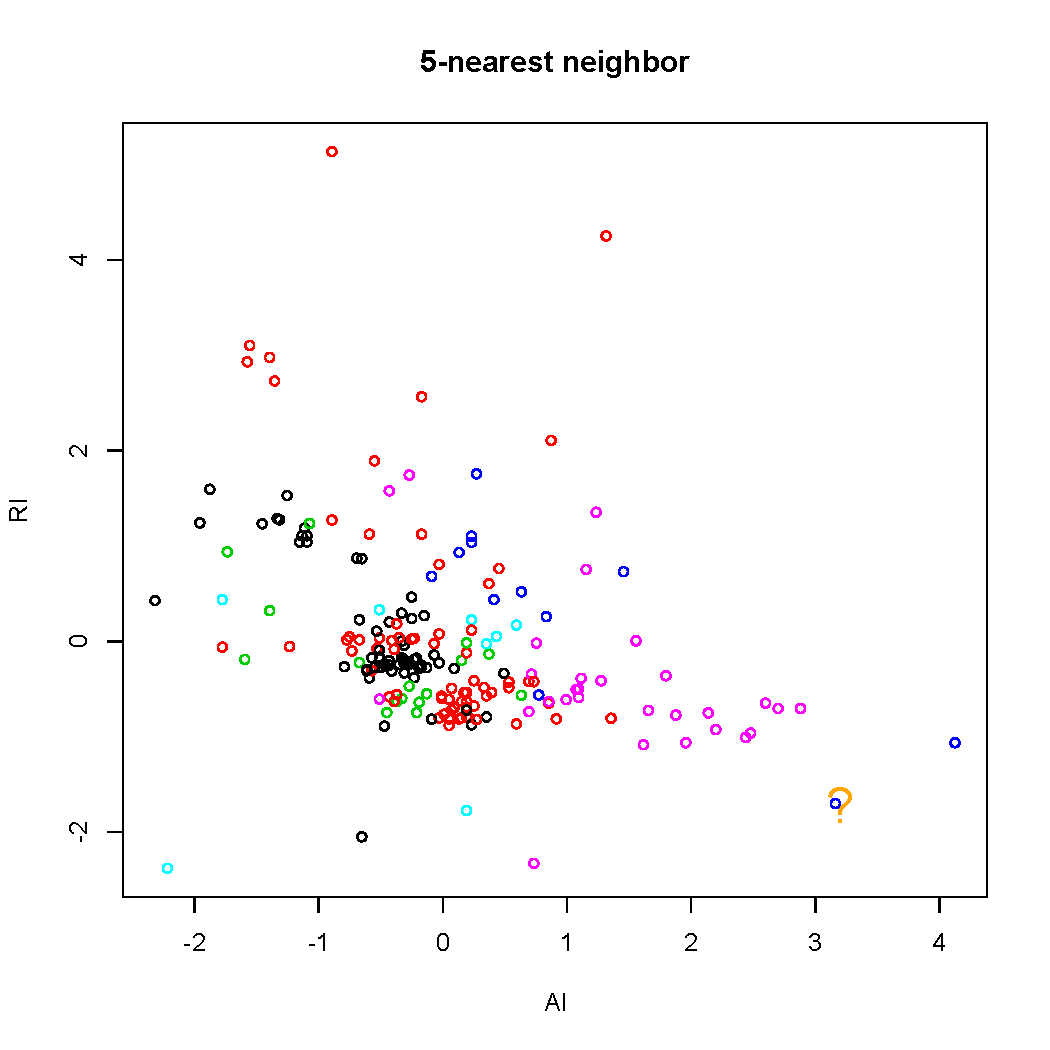
\includegraphics[width=3.5in]{knn3}
\end{center}

\end{frame}

%%%%%%%%%%%%%%%%%%%%%%%%%%%%%%%
\begin{frame}
\frametitle{$k$-Nearest Neighbors (kNN) -- Example}

\vspace{-0.5cm}

\begin{center}
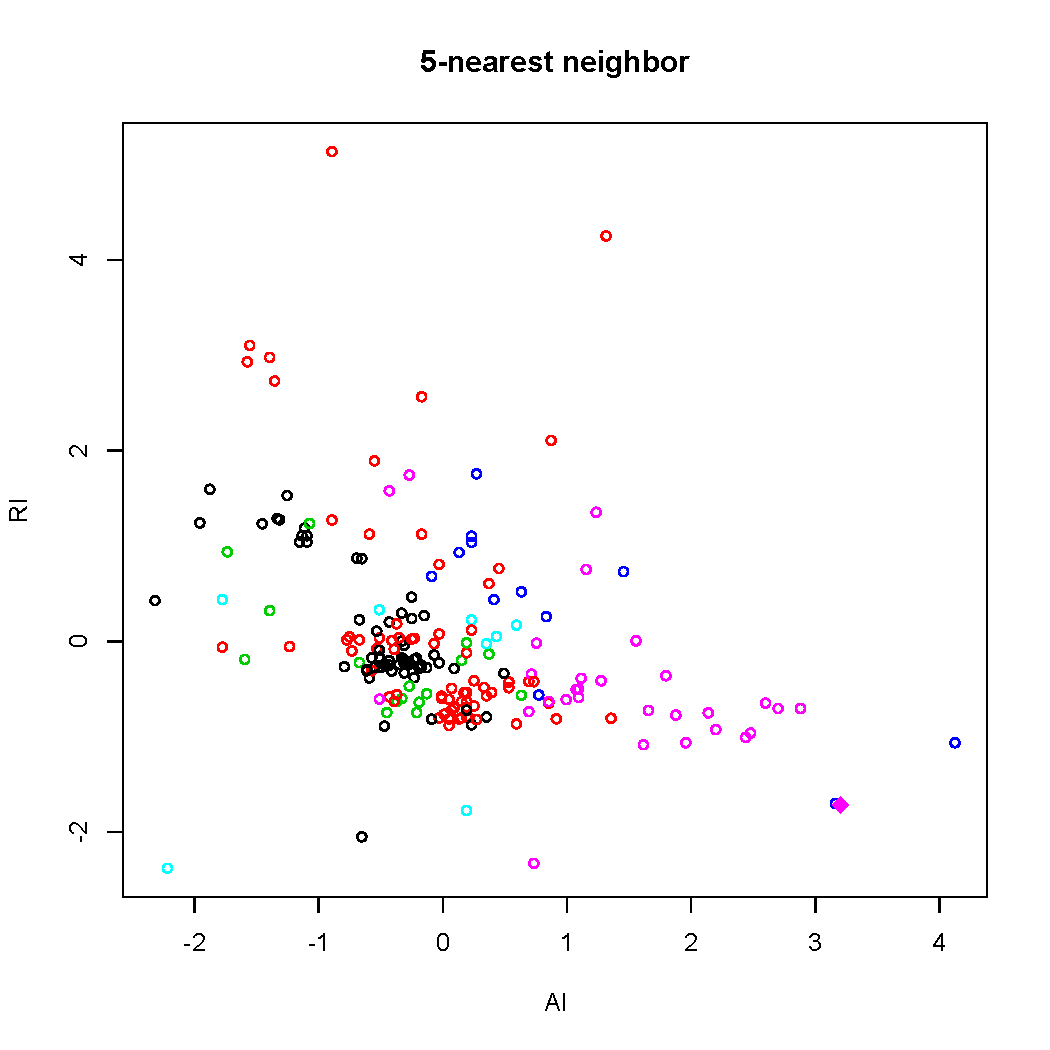
\includegraphics[width=3.5in]{knn4}
\end{center}

\end{frame}


%%%%%%%%%%%%%%%%%%%%%%%%%%%%%%%
\begin{frame}
\frametitle{$k$-Nearest Neighbors (kNN)}

{\bf Comments:}
\begin{itemize}
\item kNN is simple and intuitive and yet very powerful! {\color{red}e.g. Pandora (music genome project), Nate Silver's first company...} 
\item Choice of $k$ matters! Once again, we should rely on the out-of-sample performance
\item As always, deciding the cut-off for classification impacts the results (more on this later)
\end{itemize}
\end{frame}


%%%%%%%%%%%%%%%%%%%%%%%%%%%%%%%
\begin{frame}
\frametitle{$k$-Nearest Neighbors (kNN)}

{\bf More  comments:}
\begin{itemize}
\item The distance metric used above is only valid for numerical values of $X$. When $X's$ are categorical we need to think about a different distance metric or perform some manipulation of the information. 
\item The scale of $X$ also will have an impact. In general it is a good idea put the $X's$ in the same scale before running kNN (see example in {\tt R})
\end{itemize}
\end{frame}


%%%%%%%%%%%%%%%%%%%%%%%%%%%%%%%
\begin{frame}
\frametitle{knn: California Housing}
{\bf \color{blue}Data:} Medium home values in census tract plus the following information:
\begin{itemize}
\item Location (latitude, longitude)
\item Demographic information: population, income, etc...
\item Average room/bedroom number, home age
\item Let's start using just location as our $X's$... euclidian distance is quite natural here, right?
\end{itemize}

\skoo
{\bf \color{blue}Goal:} Predict $log(Medium Value)$ {\color{red}(why logs? more on this later)}
\end{frame}

%%%%%%%%%%%%%%%%%%%%%%%%%%%%%%%
\begin{frame}
\frametitle{knn: California Housing}
Using a training data of $n=1000$ samples, here's a picture of the results for $k=500$... {\color{red} left $\hat{Y}_i$, right $(Y_i-\hat{Y}_i)$}
\vspace{-0.8cm}
\begin{center}
\includegraphics[width=4in]{CAL500}
\end{center}
\end{frame}


%%%%%%%%%%%%%%%%%%%%%%%%%%%%%%%
\begin{frame}
\frametitle{knn: California Housing}
Now, $k=10$... does this make sense?
\vspace{-0.8cm}
\begin{center}
\includegraphics[width=4in]{CAL10}
\end{center}
\end{frame}


%%%%%%%%%%%%%%%%%%%%%%%%%%%%%%%
\begin{frame}
\frametitle{knn: California Housing}
$k$-fold cross validation... $kfold=10$
\begin{center}
\includegraphics[width=3in]{CALknn} 
\end{center}
\end{frame}



%%%%%%%%%%%%%%%%%%%%%%%%%%%%%%%
\begin{frame}
\frametitle{knn: California Housing}
Adding Income as a predictor... think about the scale of $X$... 
\begin{center}
\includegraphics[width=3in]{CALknnIcome}
\end{center}
\end{frame}


%%%%%%%%%%%%%%%%%%%%%%%%%%%%%%%
\begin{frame}
\frametitle{knn: California Housing}
Adding Income as a predictor... think about the scale of $X$...
\vspace{-0.6cm}
\begin{center}
\includegraphics[width=4in]{CALIncomek9}
\end{center}
\end{frame}






\end{document}


%%%%%%%%%%%%%%%%%%%%%%%%%%%%%%%
\begin{frame}
\frametitle{Trees}

{\bf Classification or Regression Trees} are another example of flexible, interpretable and powerful tools for prediction.

\vspace{-0.5cm}

\begin{center}
\includegraphics[width=4in]{TreeGlass}
\end{center}


\end{frame}

%%%%%%%%%%%%%%%%%%%%%%%%%%%%%%%
\begin{frame}
\frametitle{Trees}

The main idea is to split the observations in the training data into {\color{blue}subgroups} by partitioning each predictor into {\color{red}subregions}

\skoo

These partitions create a sequence of logical rules that are intuitive, interpretable and easy to visualize!

\skoo

{\bf \color{blue}Classification trees} have class probabilities at the leaves.\\
{\bf \color{blue}Regression trees} have a mean response at the leaves.


\end{frame}





%%%%%%%%%%%%%%%%%%%%%%%%%%%%%%%
\begin{frame}
\frametitle{Trees -- Glass Example}

\vspace{-0.5cm}

\begin{center}
\includegraphics[width=4.7in]{TreeGlass1}
\end{center}

\end{frame}



%%%%%%%%%%%%%%%%%%%%%%%%%%%%%%%
\begin{frame}
\frametitle{Growing Trees}

{\bf \color{red}Question:} How do we choose a tree, ie, how do we define the partitions in the space of the covariates?

\skoo

One very popular alternative is to use the {\bf CART} algorithm. It is a recursive algorithm that goes as follows:

\begin{enumerate}
\item Choose the first split among all possible splits (for every $x_i$) that minimizes $\sum_{i=1}^n(y_i - \hat{y}_i)^2$ \\{\it (or the error rate in classification trees)}

\item For each newly defined subregion, repeat step 1.

\item Stop when no new split leads to a smaller sum of squared error (or error rate)
\end{enumerate}

\skoo
\end{frame}

%%%%%%%%%%%%%%%%%%%%%%%%%%%%%%%
\begin{frame}
\frametitle{Tree Pruning: Improving prediction accuracy}

A large tree (too many terminal nodes) may {\color{red}over fit the training data}! Usual problem with very flexible, large models...

\skoo

Generally, one can improve the prediction ability of the model by ``pruning'' the tree, ie, {\color{blue}cutting down some terminal nodes}

\skoo

Again, this can (and should!) be done by comparing the out-of-sample prediction performance.

\end{frame}


%%%%%%%%%%%%%%%%%%%%%%%%%%%%%%%

\begin{frame}
\frametitle{Tree Pruning: Improving prediction accuracy}
{\color{red}Big tree Error Rate: 27\%} \ \ \ \ \ \ \ \  \ \ \  \ \ \ \ \ \ {\color{blue}Pruned Tree Error Rate: 20\%}

\includegraphics[width=4.7in]{GlassPruned}


\end{frame}

%%%%%%%%%%%%%%%%%%%%%%%%%%%%%%%
\begin{frame}
\frametitle{Trees -- Comments}

\begin{itemize}
\item Easy to {\color{blue} explain} and {\color{blue}visualize}
\item Many modifications and options to ``growing trees'' are available. For example, we might want to control the minimum number of observations in each terminal node
\item Lots of different algorithms available to grow trees
\item Can be improved by mixing over a collection of trees... Random Forests, BART... the idea is that the combination of many simple trees might do better
\end{itemize}

\end{frame}
%%%%%%%%%%%%%%%%%%%%%%%%%%%%%%%
\begin{frame}
\frametitle{California Housing}

{\bf \color{blue}Data:} Medium home values in census tract plus the following information:
\begin{itemize}
\item Location (latitude, longitude)
\item Demographic information: population, income, etc...
\item Average room/bedroom number, home age
\end{itemize}

\skoo
{\bf \color{blue}Goal:} Predict $log(Medium Value)$ {\color{red}(why logs?)}

\skoo

Would a linear model be appropriate here? Should the effect of each covariate be the same everywhere?

\end{frame}

%%%%%%%%%%%%%%%%%%%%%%%%%%%%%%%
\begin{frame}
\frametitle{California Housing}

{\bf \color{blue}Models:} Let's compare the performance of the following models:
\begin{itemize}
\item Regression: LASSO plus interactions
\item Regression Trees
\item Random Forest
\end{itemize}

\end{frame}


%%%%%%%%%%%%%%%%%%%%%%%%%%%%%%%
\begin{frame}
\frametitle{California Housing: LASSO}

\vspace{-0.5cm}

\begin{center}
\includegraphics[width=3.6in]{caPath}
\end{center}
It chooses a very large model!

\end{frame}

%%%%%%%%%%%%%%%%%%%%%%%%%%%%%%%
\begin{frame}
\frametitle{California Housing: LASSO}

\vspace{-1cm}

\begin{center}
\includegraphics[width=3.8in]{resLASSO}
\end{center}

What do you see here... any patterns?

\end{frame}

%%%%%%%%%%%%%%%%%%%%%%%%%%%%%%%
\begin{frame}
\frametitle{California Housing: Tree}

\vspace{-0.5cm}

\begin{center}
\includegraphics[width=4.8in]{caTree}
\end{center}

\end{frame}


%%%%%%%%%%%%%%%%%%%%%%%%%%%%%%%
\begin{frame}
\frametitle{California Housing: Tree}

\vspace{-1cm}

\begin{center}
\includegraphics[width=3.8in]{resTree}
\end{center}

any better?

\end{frame}
%%%%%%%%%%%%%%%%%%%%%%%%%%%%%%%
\begin{frame}
\frametitle{California Housing: Random Forest}

\vspace{-1cm}

\begin{center}
\includegraphics[width=3.8in]{resRF}
\end{center}

Now?

\end{frame}




%%%%%%%%%%%%%%%%%%%%%%%%%%%%%%%
\begin{frame}
\frametitle{California Housing: Out-of-Sample Performance}

\vspace{-1cm}

\begin{center}
\includegraphics[width=3.7in]{caMSE}
\end{center}

\end{frame}









\end{document}